\documentclass{article}

% if you need to pass options to natbib, use, e.g.:
\PassOptionsToPackage{numbers, compress}{natbib}
% before loading nips_2018

% ready for submission
\usepackage{nips_2018}

% to compile a preprint version, e.g., for submission to arXiv, add
% add the [preprint] option:
%\usepackage[preprint]{nips_2018}

% to compile a camera-ready version, add the [final] option, e.g.:
% \usepackage[final]{nips_2018}

% to avoid loading the natbib package, add option nonatbib:
% \usepackage[nonatbib]{nips_2018}

\usepackage[utf8]{inputenc} % allow utf-8 input
\usepackage[T1]{fontenc}    % use 8-bit T1 fonts
\usepackage{hyperref}       % hyperlinks
\usepackage{url}            % simple URL typesetting
\usepackage{booktabs}       % professional-quality tables
\usepackage{amsfonts}       % blackboard math symbols
\usepackage{nicefrac}       % compact symbols for 1/2, etc.
\usepackage{microtype}      % microtypography
\usepackage{algorithm}
\usepackage{algpseudocode}
\usepackage{wrapfig}
\usepackage{subcaption}

\usepackage{caption}
%\captionsetup[table]{position=bottom}

\usepackage{array}
\usepackage{epsfig}
\usepackage{epstopdf}
\usepackage{amsmath}

\begingroup
  \catcode`\_=\active
  \gdef_#1{\ensuremath{\sb{\mathrm{#1}}}}
\endgroup
\mathcode`\_=\string"8000
\catcode`\_=12

\usepackage{xcolor}
\usepackage{textcomp}
\definecolor{Gray}{rgb}{0.5,0.5,0.5}
\definecolor{darkblue}{rgb}{0,0,0.7}
\definecolor{orange}{rgb}{1,.5,0} % something readable but different from todo
\definecolor{red}{rgb}{1,0,0} % something readable but different from todo
\newcommand{\heading}[1]{\noindent\textbf{#1}}
\newcommand{\note}[1]{{\em{\textcolor{orange}{#1}}}}
\newcommand{\todo}[1]{{\textcolor{darkblue}{TODO: #1}}}
\newcommand{\changed}[1]{{\textcolor{blue}{#1}}}

\newcommand{\Matrix}[1]     {{\ensuremath{\mathbf{\uppercase{#1}}}}} %Matrix 
\newcommand{\Vector}[1]     {{\ensuremath{\mathbf{\lowercase{#1}}}}} %Vector
\newcommand{\Variable}[1]   {{\ensuremath{\mathrm{\lowercase{#1}}}}} %Scalar
\newcommand{\Id}            {\mathbb{I}} %Identity matrix

\newcommand{\mini}[1]   {\underset{{#1}}{\operatorname{min}} \: \: } %Minimize w.r.t.
\newcommand{\minimize}[1]   {\underset{{#1}}{\operatorname{argmin}} \: \: } %Minimize w.r.t.
\newcommand{\subjectto}     {\operatorname{subject to}}

\newcommand{\signal} {\Vector{x}}
\newcommand{\filter} {\Vector{d}}
\newcommand{\code}   {\Vector{z}}
\newcommand{\Filter} {\Matrix{D}}
\newcommand{\mask}   {\Matrix{M}}
\newcommand{\Code}   {\Matrix{z}}
\newcommand{\surC}   {\Matrix{C}}
\newcommand{\surB}   {\Matrix{B}}
\newcommand{\matA}   {\Matrix{A}}
\newcommand{\ite}	 {t}


\title{Stochastic Convolutional Sparse Coding}

% The \author macro works with any number of authors. There are two
% commands used to separate the names and addresses of multiple
% authors: \And and \AND.
%
% Using \And between authors leaves it to LaTeX to determine where to
% break the lines. Using \AND forces a line break at that point. So,
% if LaTeX puts 3 of 4 authors names on the first line, and the last
% on the second line, try using \AND instead of \And before the third
% author name.

\author{
  David S.~Hippocampus\thanks{Use footnote for providing further
    information about author (webpage, alternative
    address)---\emph{not} for acknowledging funding agencies.} \\
  Department of Computer Science\\
  Cranberry-Lemon University\\
  Pittsburgh, PA 15213 \\
  \texttt{hippo@cs.cranberry-lemon.edu} \\
  %% examples of more authors
  %% \And
  %% Coauthor \\
  %% Affiliation \\
  %% Address \\
  %% \texttt{email} \\
  %% \AND
  %% Coauthor \\
  %% Affiliation \\
  %% Address \\
  %% \texttt{email} \\
  %% \And
  %% Coauthor \\
  %% Affiliation \\
  %% Address \\
  %% \texttt{email} \\
  %% \And
  %% Coauthor \\
  %% Affiliation \\
  %% Address \\
  %% \texttt{email} \\
}

\begin{document}
% \nipsfinalcopy is no longer used

\maketitle


\begin{abstract}

\end{abstract}

\section{Introduction}
Convolutional Sparse Coding (CSC) is a method for learning {\em
  generative} models in the form of translationally invariant
dictionaries for a large variety of different training signals.  These
generative models have been shown effective for solving problems in
neural and brain information
processing~\cite{jas2017learning,peter2017sparse}, as well as in a
variety of image processing tasks, for instance, image
inpainting~\cite{heide2015fast},
super-resolution~\cite{gu2015convolutional}, high dynamic range
imaging~\cite{serrano2016convolutional}, and high-dimensional signal
reconstructions~\cite{choudhury2017consensus,bibi2017high}. CSC
differs from conventional sparse coding by formulating the signals as
the sum of a set of convolutions on dictionary filters and sparse
codes instead of patch-wise linear combinations of
filters. In traditional sparse dictionary learning, the patch
structure significantly degrades the expressiveness of the
dictionaries by introducing a strong dependency on the position of a
feature, which the convolutional nature of CSC avoids.
%% Alternatively, sparse coding, as a patch-based approach,              %%
%% learns filters from partitioned local structures, and this partition  %%
%% manipulation discards inherent correlations between those patches, so %%
%% as to learns redundant filters (the same or similar ones with         %%
%% translated versions). Owing to the convolutional property, the        %%
%% dictionary learned from CSC achieves signal global coherence, tending %%
%% to be more representative.                                            %%

\changed{This convolutional approach is also at the heart of many deep
learning-based methods in the form of
CNNs~\cite{lecun1998gradient,kavukcuoglu2010learning,krizhevsky2012imagenet},
which have in recent years been extraordinarily successful for a broad
range of high-level image understanding applications. However, while
CNNs generally are used in a {\em supervised} setting and produce {\em
  discriminative}, task-specific models, CSC is {\em unsupervised} and
produces {\em generative} models that can easily be transferred between tasks.}

To solve the optimization problems inherent to CSC, Zeiler et
al.~\cite{zeiler2010deconvolutional} iteratively solve two subproblems
(updating sparse codes and updating filters) using gradient decent in
the form of convolutional operations in the spatial domain, which is
computationally expensive. Recent algorithms tackle the problem by
exploiting Parseval's theorem to express the spatial convolution by
multiplication in the frequency domain and using proximal solver such
as Alternating Direction Method of Multipliers
(ADMM)~\cite{boyd2011distributed} to separate the linear least squares
parts from the non-smooth terms in the optimization
problem. These approaches show tremendous improvements over prior
spatial-domain solvers with respect to running
time~\cite{bristow2013fast,heide2015fast,wohlberg2016efficient,choudhury2017consensus}. Most
of the prior work learns the dictionary filters in a batch mode, which
indicates that all training signals are involved in every training
iteration, and this restricts it from applying to large datasets or
streaming data.

In contrast to batch mode learning, online
learning~\cite{shalev2012online} is a well established strategy which
processes a single image or a small portion (mini-batch) of the whole
data at each training step, and incrementally updates model
variables. Herein, the required memory and computing sources are only
dependent on the sample size in every observation, independent of the
training data size. It alleviates the scalability issue that arises in
batch approaches, and the convergence of the algorithm was firstly
analyzed using stochastic approximation
tools~\cite{bottou1998online}. Bottou et
al.~\cite{bousquet2008tradeoffs} further showed better generalization
performance of the stochastic algorithms than standard gradient
descent on large scale learning systems. Later on, online learning
strategies were synergetic with sparse coding, which was then scaled
up for learning dictionary from millions of training
samples~\cite{mairal2009online,mairal2010online}, and for large-scale
matrix factorization with an additionally introduced subsampling
strategy~\cite{mensch2016dictionary}. More recently, Liu et
al.~\cite{liu-2018-first} and Wang et al.~\cite{wang2018scalable}
separately proposed similar online learning frameworks for the CSC
model, alleviating the memory issues arise in batch-based CSC model on
large datasets.

{\bfseries Contributions.} \changed{We mainly make three contributions in this
work. First, we introduce a randomization strategy for the CSC
model and solve the entire problems in the spatial domain. We demonstrate
that the proposed stochastic spatial-domain solver, with a reasonably
selected subsampling rate, outperforms the state-of-the-art
frequency-domain solvers with regard to computing efficiency. Secondly, we
formulate an online-learning version of the proposed algorithm, and
show dramatic runtime improvement over current online CSC methods,
while producing comparable outcomes. Finally, we demonstrate the
capability to learn the meaningful over-complete dictionary from thousands of
images, and analyze the effectiveness of the learned over-complete
dictionary for a number of reconstruction tasks.}


% --- DO NOT DELETE ---
% Local Variables:
% mode: latex
% mode: flyspell
% mode: TeX-PDF
% End:



\section{Convolutional Sparse Coding (CSC)} \label{CSCmodel}
The dictionary learning problem for CSC problem has the form
\begin{equation}\label{eq:CSCmodel}
\begin{split}
    \mini{\filter,\code} & \frac{1}{2}\|\signal - \sum_{k=1}^{K} \filter_k * \code_k \|_2^2 + \lambda \sum_{k=1}^{K}\| \code_k \|_1 \\
    \text{subject to} & ~ \|\filter_k\|^2_2 \leq 1 ~~ \forall k \in \{1,\dots,K\},
\end{split}
\end{equation}
where $\signal \in \mathbb{R}^D$ is a $D$-dimensional signal or a
vectorized image,
$\filter_k \in \mathbb{R}^M$ is the $k$-th dictionary, $\code_k\in
\mathbb{R}^D$ is the sparse code associated with that dictionary,
$\lambda>0$ is a sparsity inducing penalty parameter, $K$ is the
number of dictionary filters, and $*$ is the convolution operator. The
above model will be applied to all the training images
$\signal\in\mathbb{X}$.

Most recent CSC algorithms exploit Parseval's theorem and introduce
two slack variables to separate the non-smooth $L_1$ penalty term and
the $L_2$ constraints, making it feasible to efficiently compute the
latter in the frequency domain. Furthermore, the whole
Problem~\eqref{eq:CSCmodel} can be split into alternating subproblems
for updating $\code$ and $\filter$, which are jointly solved by
coordinate
descent~\cite{bristow2013fast,heide2015fast,wohlberg2016efficient}. This
approach suffers from several issues:

\begin{itemize}
  \item While CSC overcomes the independence assumption held in
    patch-based learning algorithms, far more variables ($K$ times
    more) are introduced to represent a single image to compensate for
    this. This creates more severe memory and computational burdens.

  \item We observe through experiments that the vast majority of the
    entries of the reconstructed sparse codes do not provide useful
    information about the represented image. For $K=100$, 99.5\%
    entries are not informative. This indicates that the subproblem
    for updating $\code$ solves a highly sparse LASSO
    problem. Transforming the problem into frequency domain imposes
    restrictions on exploiting this sparsity.

  \item While prior work shows its efficiency in solving the CSC
    problem in the frequency domain, this is only applicable for
    updating $\code$, and does not hold for updating $\filter$. The
    dictionary filters usually have much smaller spatial support than
    the dimension size of the sparse codes ($M \ll D$). However, in
    order to tackle the problem in the frequency domain, it is
    necessary to process the $\filter$-subproblem over the full
    support of the sparse codes, and then project the results onto the
    much smaller spatial support of the filters.
\end{itemize}


% --- DO NOT DELETE ---
% Local Variables:
% mode: latex
% mode: flyspell
% mode: TeX-PDF
% End:



\section{Stochastic Convolutional Sparse Coding}
\subsection{The Model}
Based on the specific sparsity property of the codes, we propose a variant of the CSC model using subsampling strategy,
and formulate the following modified minimization problem:
\begin{align}
    &\minimize{\filter,\code}  \frac{1}{2}\|\signal - \sum_{k=1}^{K} \filter_k * \mathcal{M}_k(\code_k) \|_2^2 + \lambda \sum_{k=1}^{K}\| \mathcal{M}_k(\code_k) \|_1  \nonumber \\
    &\text{subject to} ~ \|\filter_k\|^2_2 \leq 1 ~~ \forall k \in \{1,\dots,K\},
\end{align}
where $\mathcal{M}_k(\code_k)$ is the operation to subsample the corresponding code $\code_k$ following a Bernoulli distribution with probability $p$. The probability $p$ controls the fraction of the sparse codes that will be considered by the solver, and in the case of $p=1$, the proposed model is identical with the classical CSC model. If $p<1$, the algorithm only solves the sparse codes at chosen positions in each iteration, and accordingly, the update of dictionary $d$ is based on the selected portion of the sparse codes. Similar to solving the classical CSC problem, we can apply coordinate descent algorithm, alternating on subproblems of $\mathcal{M}(\code)$ and $\filter$, to solve the above optimization problem. Specifically, the modified minimization problem for $\code$ can be formulated as:
\begin{equation} \label{eq:updatingCode}
    \code_{opt} = \minimize{\code} \frac{1}{2}\|\signal - (\Filter \mask^\top)(\mask \code) \|_2^2 + \lambda \|\mask \code\|_1,
\end{equation}
where $\Filter = [\Filter_1, \dots, \Filter_K] \in \mathbb{R}^{D \times DK}$, $\code = [\code_1, \dots, \code_K] \in \mathbb{R}^{DK}$, the convolution operator are formulated in matrix multiplication so that $ \Filter \code = \sum_{k=1}^{K} \filter_k * \code_k$.  Matrix $\mask$ is a $\mathbb{R}^{pDk \times DK}$ random diagonal matrix with ones on the entries corresponding to the sampled sparse codes and zeros elsewhere, performing the function of $\mathcal{M}(\code)$. Due to the introduced subsampling matrix, the convolution operator will not hold, hence it cannot be directly solved in the frequency domain. Owing to the subsampling strategy, the number of variables that needs to be computed for this subproblem is $pDK$ instead of $DK$, and this can lead to a reduction of the computation time up to a factor of $\frac{1}{p}$ when solving it in spatial domain.

After obtaining the subsampled sparse codes, we can then project them onto its original spatial support with $0$ filling. Afterwards, the dictionary can be updated by:
\begin{equation} \label{eq:updatingFilter}
\begin{split}
   & \filter_{opt} = \minimize{\filter} \frac{1}{2}\|\signal - \Code \filter \|_2^2 \\
   & \text{subject to}  ~ \|\filter_k\|^2_2 \leq 1 ~ \forall k \in \{1,\dots,K\},
\end{split}
\end{equation}
where $\Code= [\Code_1, \dots, \Code_K] \in \mathbb{R}^{D \times MK}$ is a concatenated matrix, and $\Code_k$ is constructed from the associated $\code_k$, $\filter= [\filter_1,\dots,\filter_K] \in \mathbb{R}^{MK}$ such that $ \Code \filter = \sum_{k=1}^{K} \filter_k * \code_k$. In the common settings for CSC problem, $M \ll D$, hence there is no need to perform subsampling on dictionary.

The work of~\cite{mensch2016dictionary} also applies the stochastic subsampling strategy for dictionary learning, while the subsampling is randomly performed on the observed data, differing from that of our proposed. One can think of our proposed randomization approach as a variant of the stochastic Frank-Wolfe algorithm~\cite{reddi2016stochastic,pmlr-v80-kerdreux18a}, in which a subset of the variables are randomly extracted based on a certain probability distribution at each iteration. For the proposed algorithm, each iteration extracts ($pDK+MK$) variables, where $pDK$ variables are randomly picked out from $DK$ variables with identical probability and the rest remain unchanged. Owing to the highly sparse codes, the original signals can still be represented by a portion of the codes with a reasonable subsampling rate. Herein, unlike the stochastic Frank-Wolfe algorithm that generally requires more iterations to reach convergence, the convergence of the proposed algorithm will not be significantly affected by the subsampling manipulation. This will be experimentally verified in Section~\ref{sec:result}.

The proposed subsampling strategy will be implemented in the fashions of {\em batch mode} (stochastic batch CSC) and {\em online mode} (stochastic online CSC).

\subsection{Stochastic Batch CSC (SBCSC)}
We first formulate the batch-mode of the proposed method as shown in Algorithm~\ref{algo:SBCSC}, where $N$ is the number of total input images, $\code^i$ is the sparse code associated with $i$-th image, and $p$ is the uniform probability for one code been selected. We choose $p=\{1, 0.5, 0.2, 0.1, 0.05\}$ for testing in this work, where $p=1$ indicates no subsampling, and $p=0.05$ indicates a subsampling rate of $5\%$. Problem~\ref{eq:updatingCode} is the standard LASSO, which can be solved by plenty of optimization frameworks. We found that solving it by ADMM delivers a good balance for computation time and convergence within a moderate number of iterations. Specifically, the data fitting term and the $L_1$ penalty term are split, forming two separate substeps. The first substep is a quadratic programming (QP) problem, and we can either cache the matrix factorization by Cholesky decomposition (when $N$ is relatively large), or solve it by Conjugate Gradient (when $N$ is relatively small). The second substep can be solved by a point-wise shrinkage operation. Problem~\ref{eq:updatingFilter} is a quadratic constrained quadratic programming (QCQP) problem, and it can be efficiently solved by projected block coordinate decent. Empirically, a single iteration is enough with $\filter$ computed in previous iteration as a warm start. We set the hyperparameters $\lambda=1$, the ADMM iteration fixed to 10, the augmented Lagrangian penalty $\rho$ to $10 \lambda$, and the over-relaxation strategy within ADMM is applied with $\alpha = 1.8$. For a detailed description of the above two solvers, please refer to the supplement.

Every outer loop of SBCSC involves all of the training images, thus it would be computationally expensive to process them simultaneously and also runs out of memory quickly with the increase of the number of images. The batch-based learning algorithm lacks of the capability to scale up to very large datasets or to handle dynamically changed training data.

\begin{algorithm}[H]
\caption{SBCSC} \label{algo:SBCSC}
\begin{algorithmic}[1]
\State $\text{Initialize } \filter, ~p$
\While {not converge}
    \State $ \text{Randomly sample }\code \text{ with rate } p $
    \For{i=1 to N}
        \State $ \text{Update } \code^i \text{ by solving problem~(\ref{eq:updatingCode}})$
    \EndFor
    \State $\text{Update } \filter \text{ by solving problem~(\ref{eq:updatingFilter}})$
\EndWhile
\end{algorithmic}
\end{algorithm}

\subsection{Stochastic Online CSC (SOCSC)}
We can further tackle the proposed problem in the online fashion for a gain of scalability. In the online learning setting as shown in Algorithm~\ref{algo:SOCSC}, each iteration only draws one or a subset (mini-batch) of the total training images, hence the complexity per loop is independent of the training sample size. Then, given the sampled image $\signal^t$ at $t$-th iteration, we can compute the corresponding subsampled sparse codes $\code^t$ by
\begin{equation} \label{eq:updatingCodeOnline}
    \code^t = \minimize{\code} \frac{1}{2}\|\signal^t - (\Filter^{t-1} (\mask^t)^\top)(\mask^t \code) \|_2^2 + \lambda \|\mask^t \code\|_1,
\end{equation}
where $\Filter^{t-1}$ is constructed from the dictionary learned by $(t-1)$th iteration, and $\mask^t$ is the subsample matrix at current iteration. After obtaining the sparse codes, the dictionary is updated by:
\begin{equation}
\begin{split}
    &\filter^t = \minimize{\filter} \frac{1}{2t}\sum_{i=1}^{t} \|\signal^i - \Code^i \filter \|_2^2 \\
    &\text{subject to} \quad \|\filter_k\|^2_2 \leq 1 ~ \forall k \in \{1,\dots,K\}.
\end{split}
\end{equation}
Notice that updating dictionary involves all of the past training images and sparse codes. As shown in~\cite{mairal2009online,mairal2010online}, we can get rid of explicitly storing those data by introducing two surrogate matrices $\surC \in \mathbb{R}^{KM \times KM}$ and $\surB \in \mathbb{R}^{KM \times 1}$, which carry all of the required information for updating $\filter$, and can be iteratively updated by:
\begin{equation} \label{eq:updateSur}
\begin{split}
    \surC^t  = \frac{t-1}{t} \surC^{t-1} + \frac{1}{t}(\Code^t)^\top \Code^t \\
    \surB^t  = \frac{t-1}{t} \surB^{t-1} + \frac{1}{t}(\Code^t)^\top \signal^t
\end{split}
\end{equation}
If so, the updated dictionary can be obtained by solving:
\begin{equation} \label{eq:updatingFilterOnline}
\begin{split}
    & \filter^t = \minimize{\filter} \frac{1}{2} \filter^\top \surC^t\filter - \filter^\top \surB^t \\& \text{subject to} \quad \|\filter_k\|_2^2 \leq 1 ~ \forall k \in \{1,\dots,K\}.
\end{split}
\end{equation}
Problem~\ref{eq:updatingCodeOnline} and problem~\ref{eq:updatingFilterOnline} are solved in the same way as that for SBCSC.

\begin{algorithm}[H]
\caption{SOCSC} \label{algo:SOCSC}
\begin{algorithmic}[1]
\State $\text{Initialize} ~ t=0, ~\filter^t, ~p, ~\surC^t = 0, ~\surB^t = 0$
\While {not converge}
    \State $t \gets t+1$
    \State $ \text{draw } \signal^t \text{ from training images} $
    \State $ \text{Randomly sample }\code^t \text{ with rate } p $
    \State $ \text{Compute } \code^t \text{ by solving problem~(\ref{eq:updatingCodeOnline}) using } \filter^{t-1}$
    \State Compute $\surC^t$ and $\surB^t$ by eq~(\ref{eq:updateSur})
    \State Compute $\filter^t$ by solving problem~(\ref{eq:updatingFilterOnline})
\EndWhile
\end{algorithmic}
\end{algorithm}

\subsection{Complexity Analysis}
Recall that $D$ is the number of pixels for a single image, $K$ is the number of filters, and $M$ is the size of the filter support. For the state-of-the-art frequency-domain solvers, it has the time complexity $\mathcal{O}(K^2D + KDlog(D))$ for a single data pass. 

Compared with SBCSC, updating $\code$ (suppose we solve it by Conjugate Gradient) has the time complexity of $\mathcal{O}(pKMD \sqrt{\tau})$ where $pKMD$ is the number of non-zero elements in $(\Filter \mask^\top)$ and $\tau$ is the condition number of $(A^\top A + \rho I)$ where $A = \Filter \mask^\top$. With a reasonable selection of the subsampling rate, this time complexity is comparable with that of frequency-domain solvers. As for updating $\filter$, it takes $\mathcal{O}(K^2M^2)$ time. This is comparable to $\mathcal{O}(K^2D)$ in common CSC settings ($M \ll D$), while it requires multiple iterations in frequency domain and only one pass required by the proposed method, which greatly saves the time. Overall, the proposed method has the time complexity of $\mathcal{O}(pKMD \sqrt{\tau} + K^2M^2)$.

The time complexity of SOCSC is similar to that of SBCSC, apart from two additional steps to update the surrogate matrices. Updating $\surC$ and $\surB$ involves computing $\Code^\top\Code$ and $\Code^\top x$. Though $\Code$ has the dimensions of $D \times KM$, it is a highly sparse matrix with only $\mathcal{O}(D)$ non-zero elements. Therefore, the total time complexity will not be obviously affected. 

\section{Results} \label{sec:result}
We first validate the proposed algorithms on the fruit and city
datasets~\cite{zeiler2010deconvolutional}, which each consist of 10
training images of size $100 \times 100$. The online-mode algorithms
are then adapted to one thousand $100 \times 100$ image patches
randomly picked up from ImageNet~\cite{deng2009imagenet}. Note that
batch-based CSC commonly can only handle less than 100 images
simultaneously. The dictionary size is set to $100$ filters of size
$11 \times 11$ pixels in all experiments except for over-complete
dictionary. All training and evaluation processes in this manuscript
are performed on contrast normalized
images~\cite{zeiler2010deconvolutional,heide2015fast}.

\begin{figure}[h]
\centering
\begin{subfigure}{0.5\textwidth}
  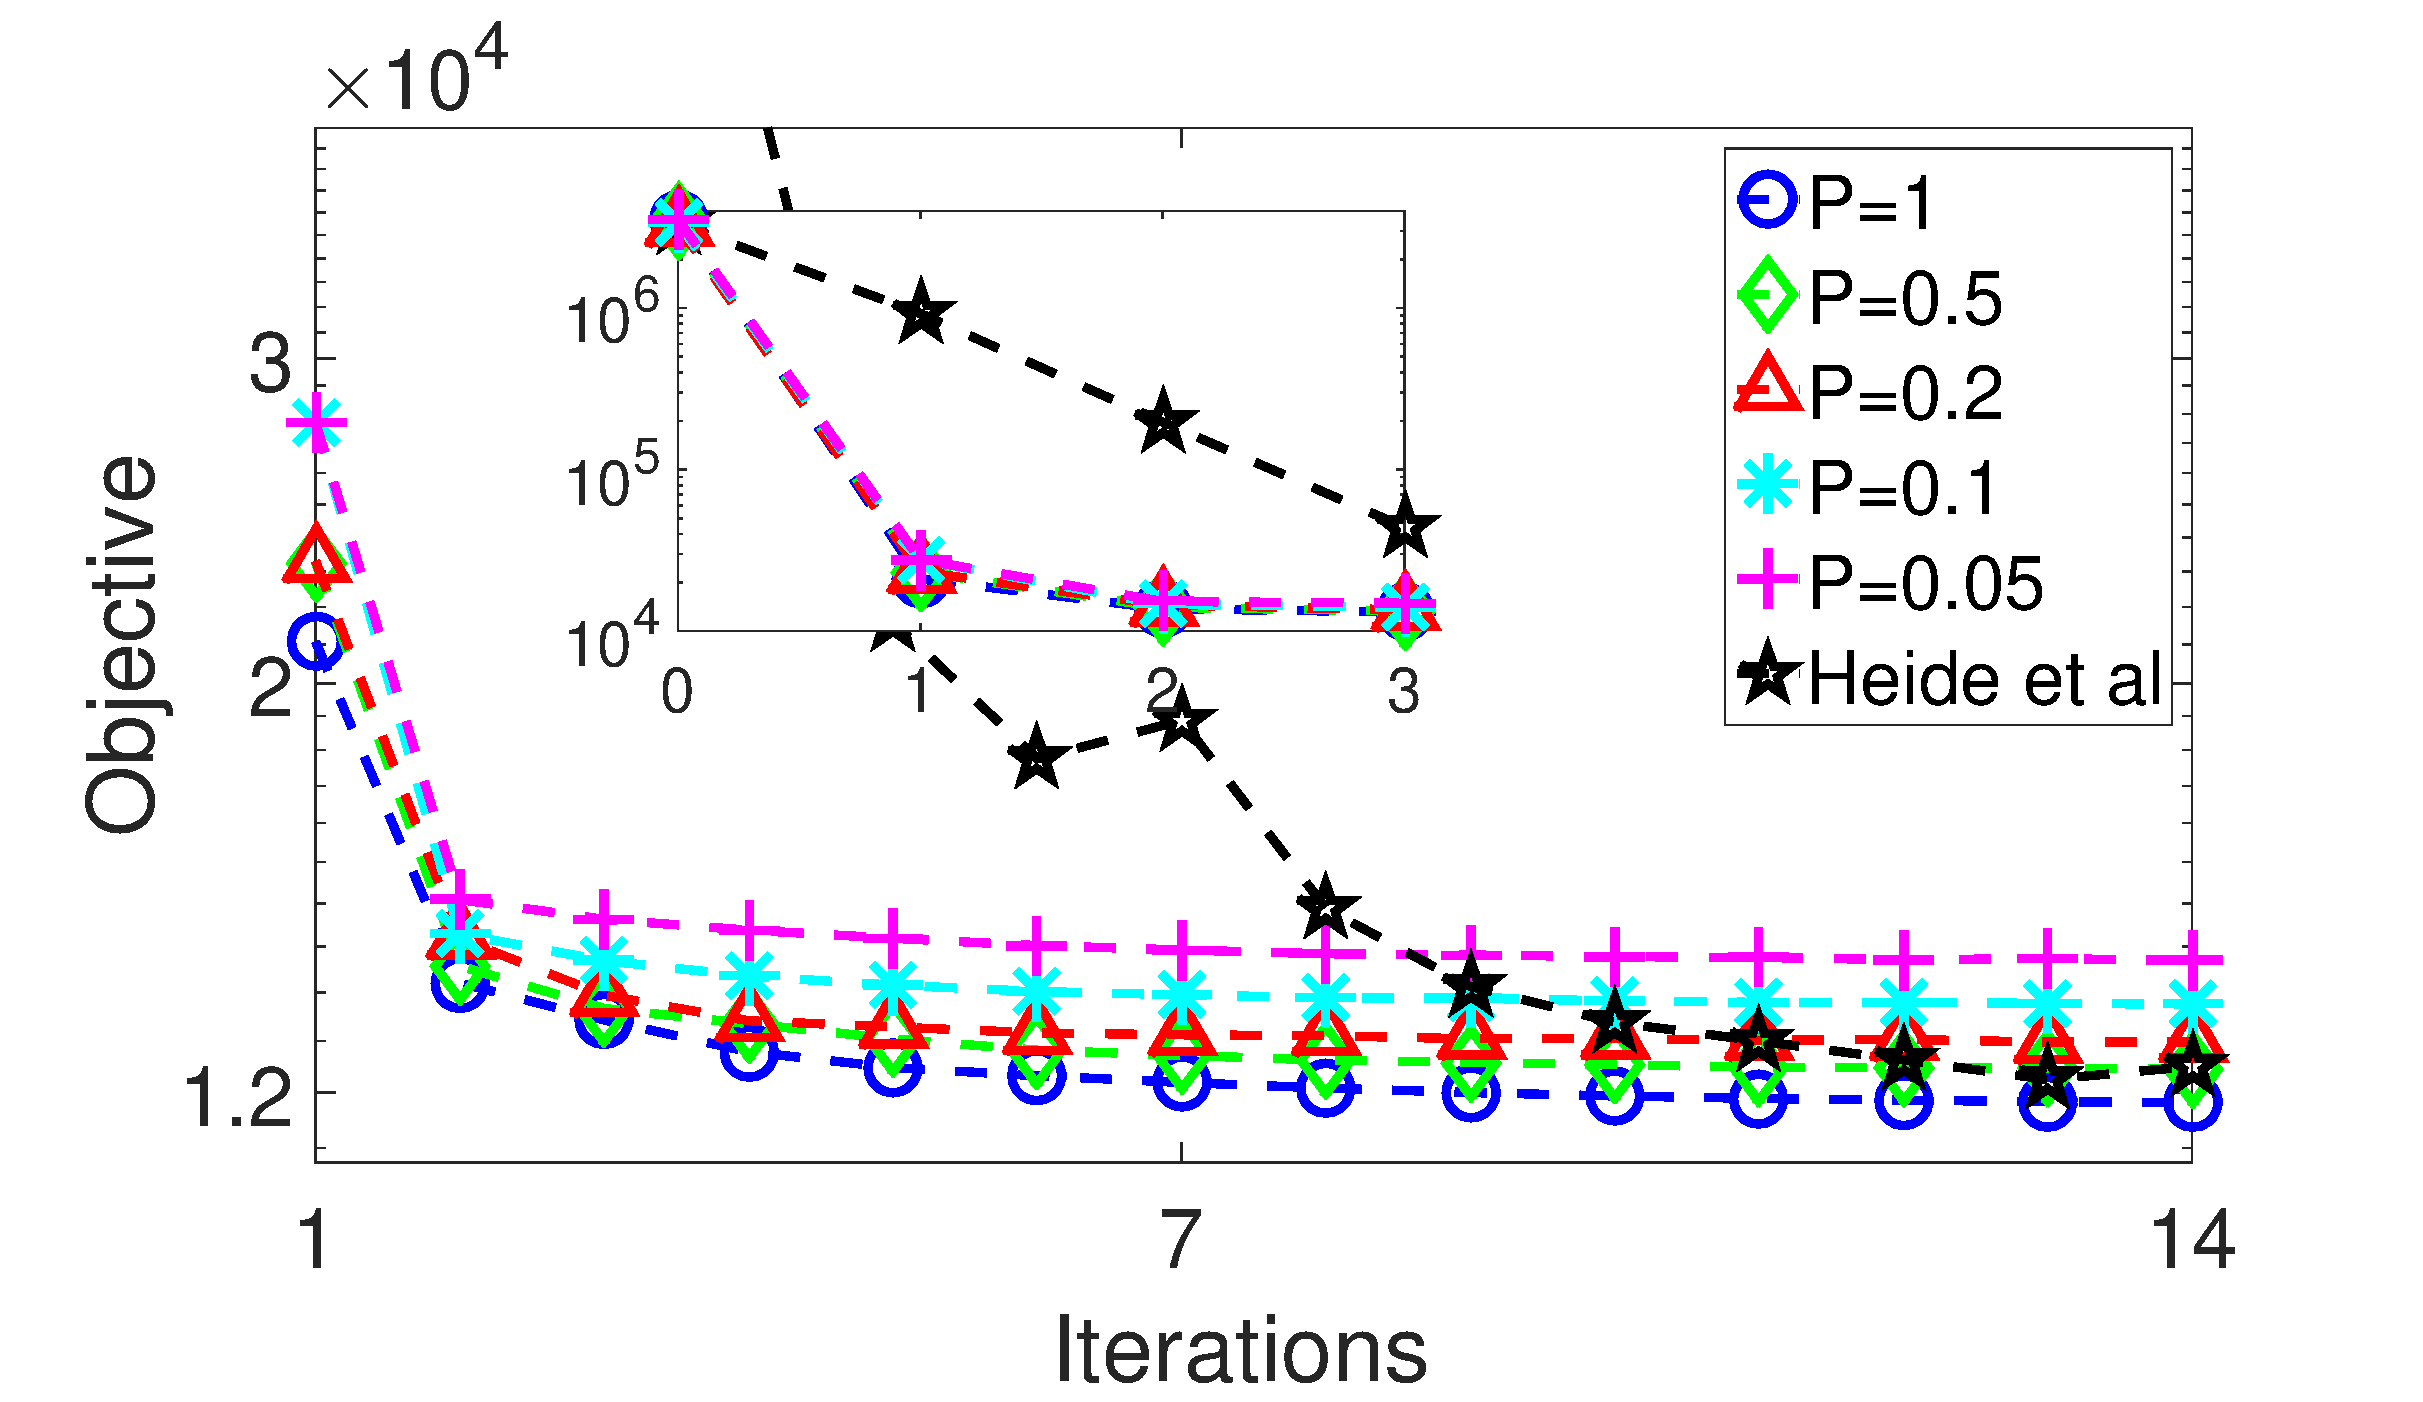
\includegraphics[width=1\linewidth]{figure/iteVSobj.pdf}
\end{subfigure}

\begin{subfigure}{0.5\textwidth}
  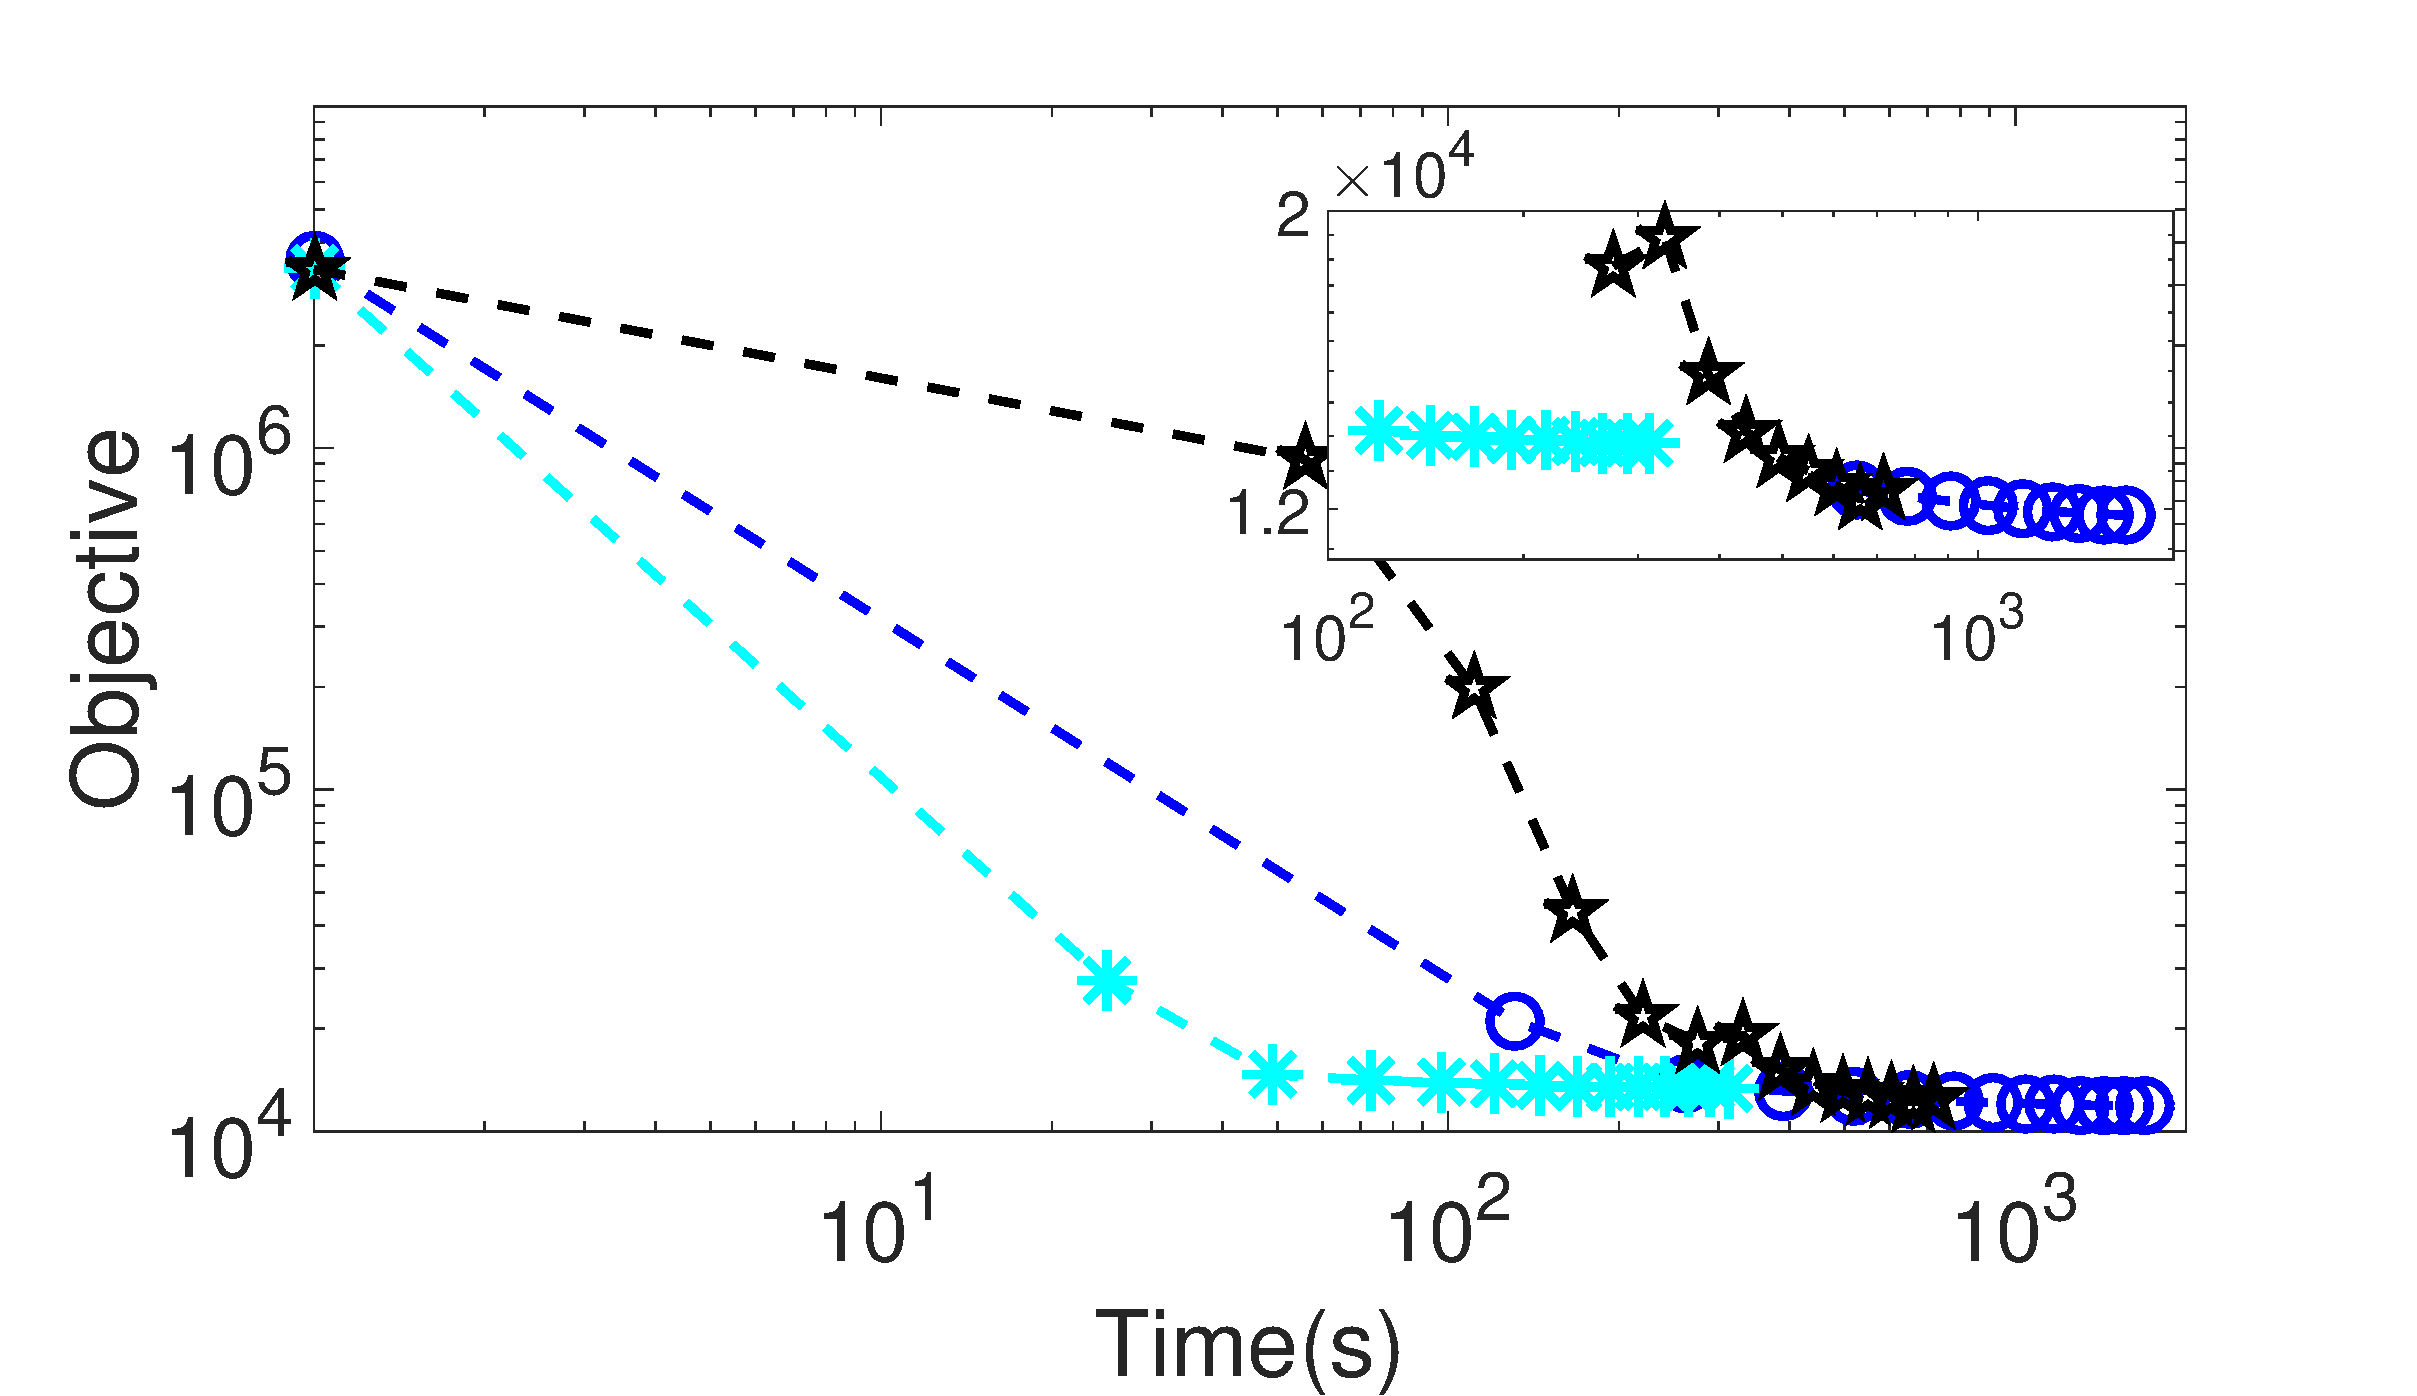
\includegraphics[width=1\linewidth]{figure/timeVSobj.pdf}
  \vspace*{1mm}
\end{subfigure}

\begin{subfigure}{0.23\textwidth}
  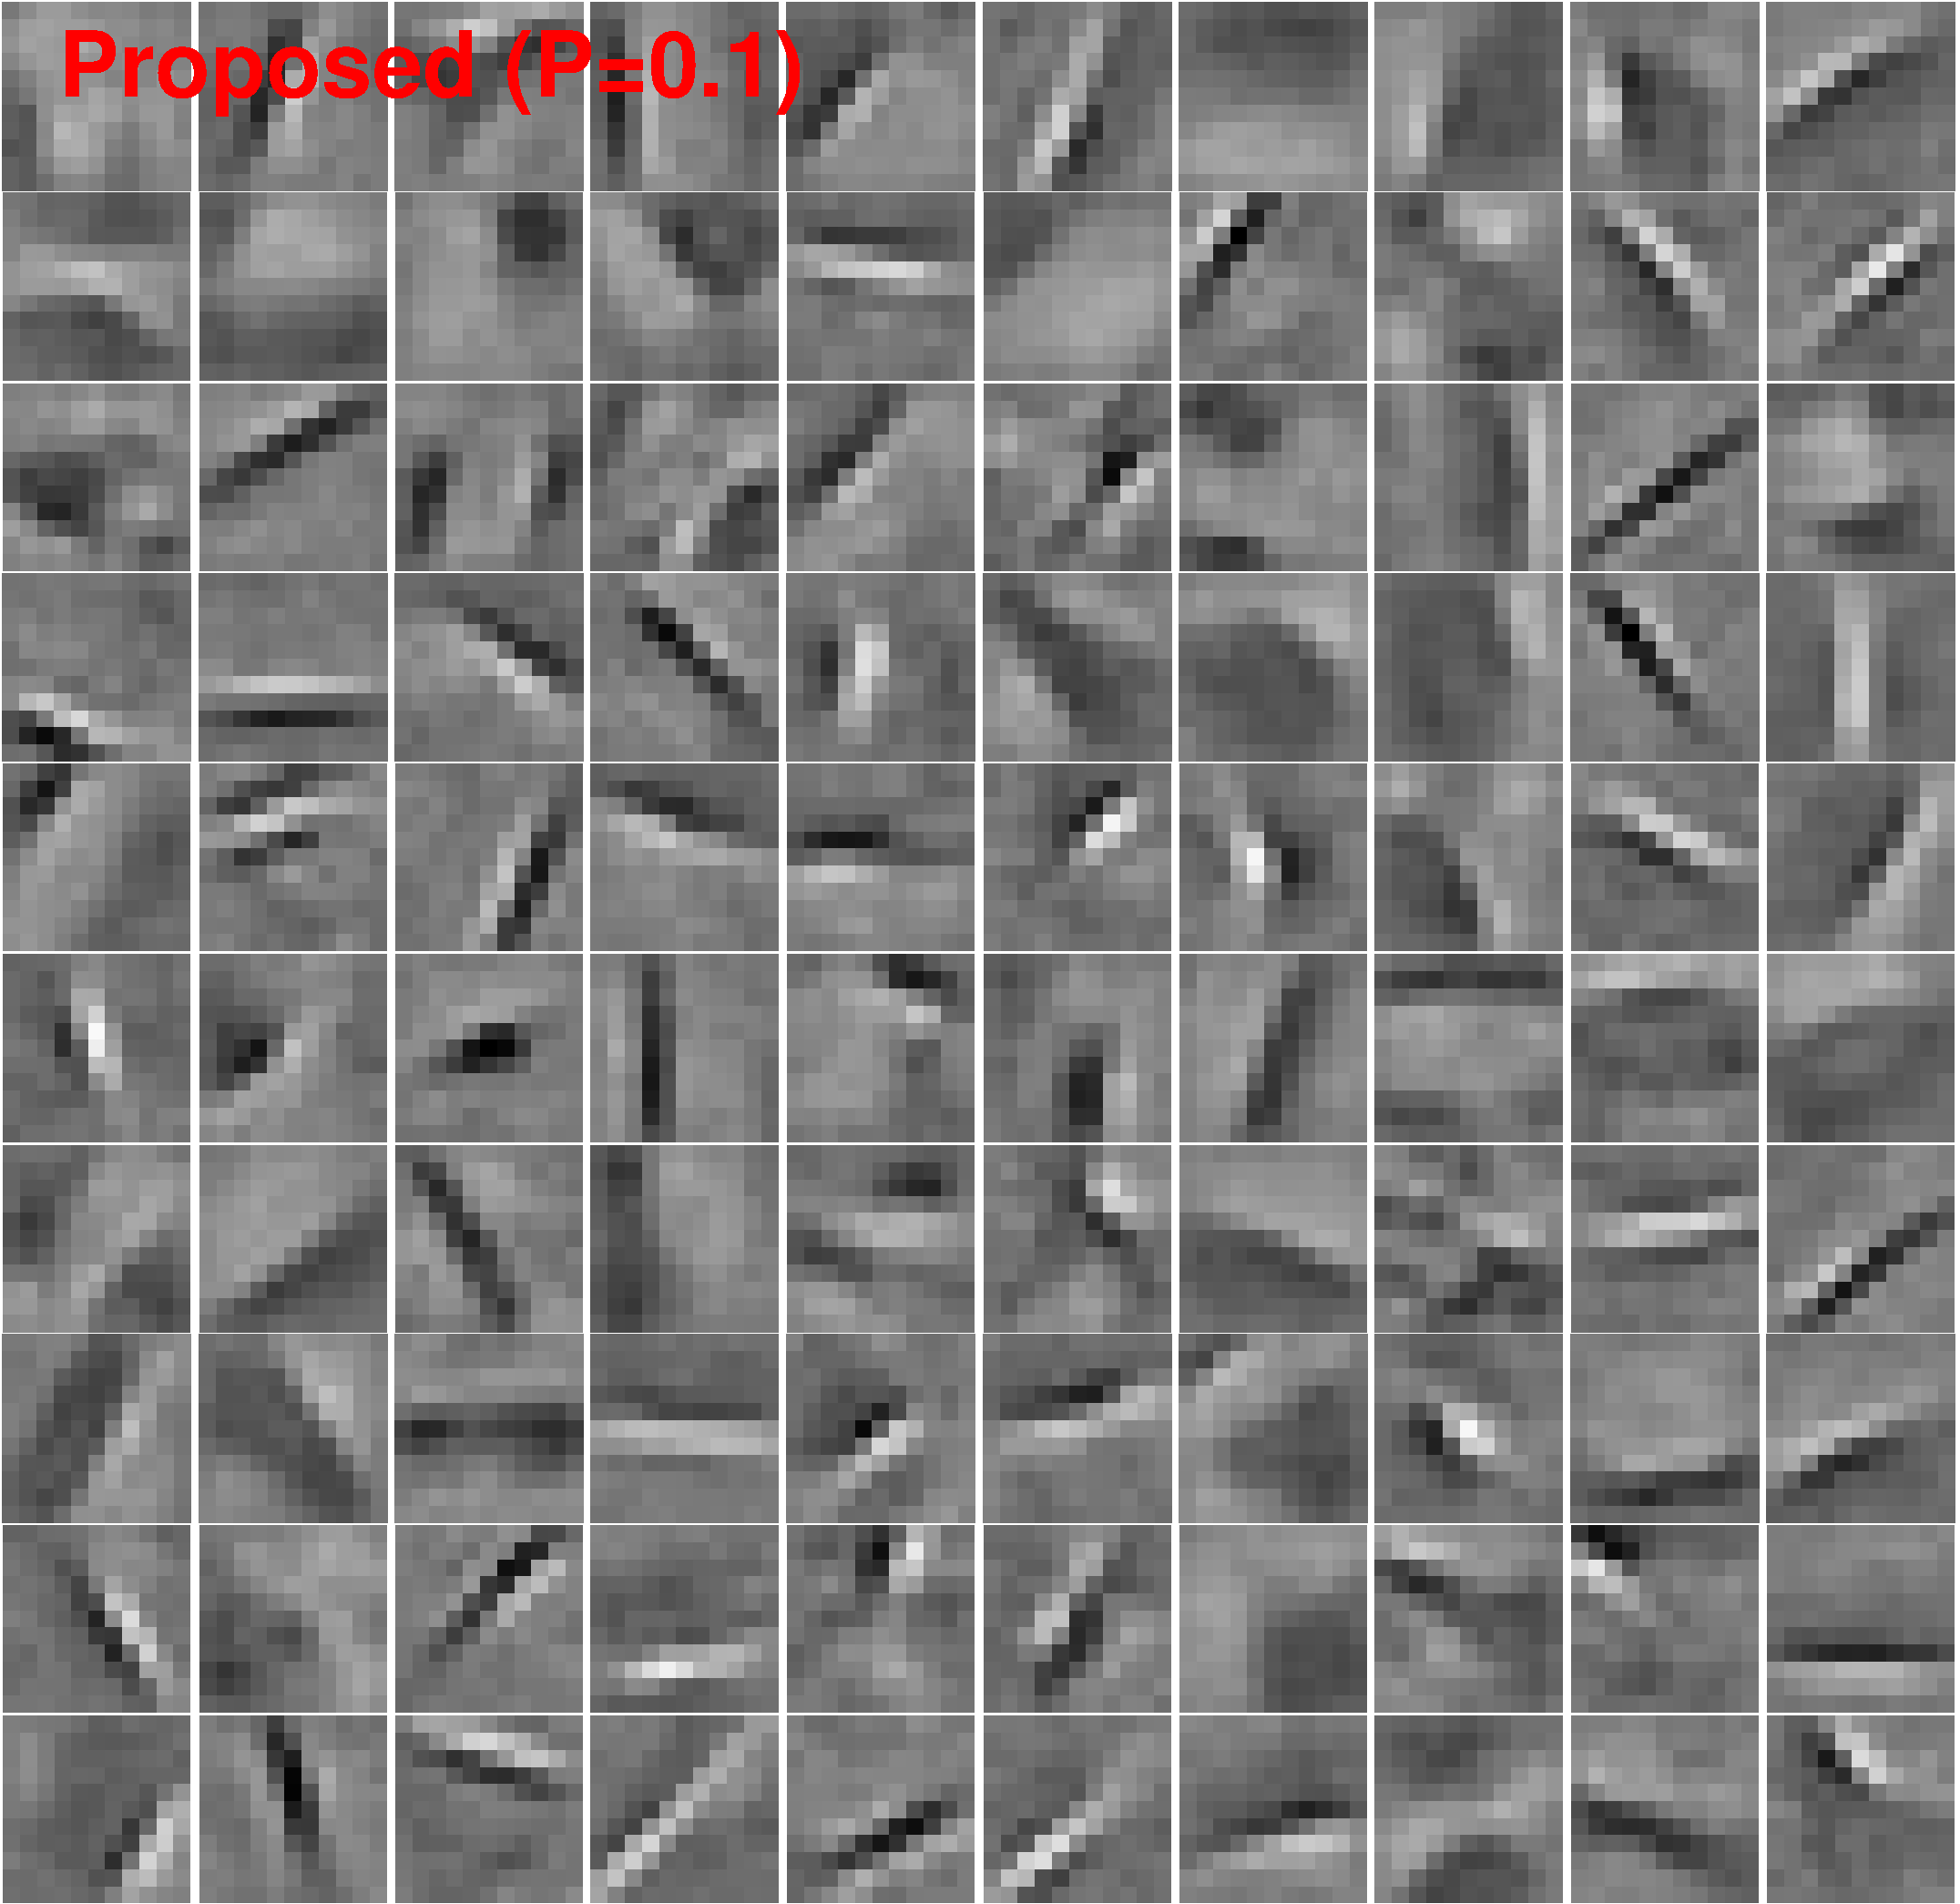
\includegraphics[width=1\linewidth]{figure/batchFruit100.pdf}
\end{subfigure}
\begin{subfigure}{0.23\textwidth}
  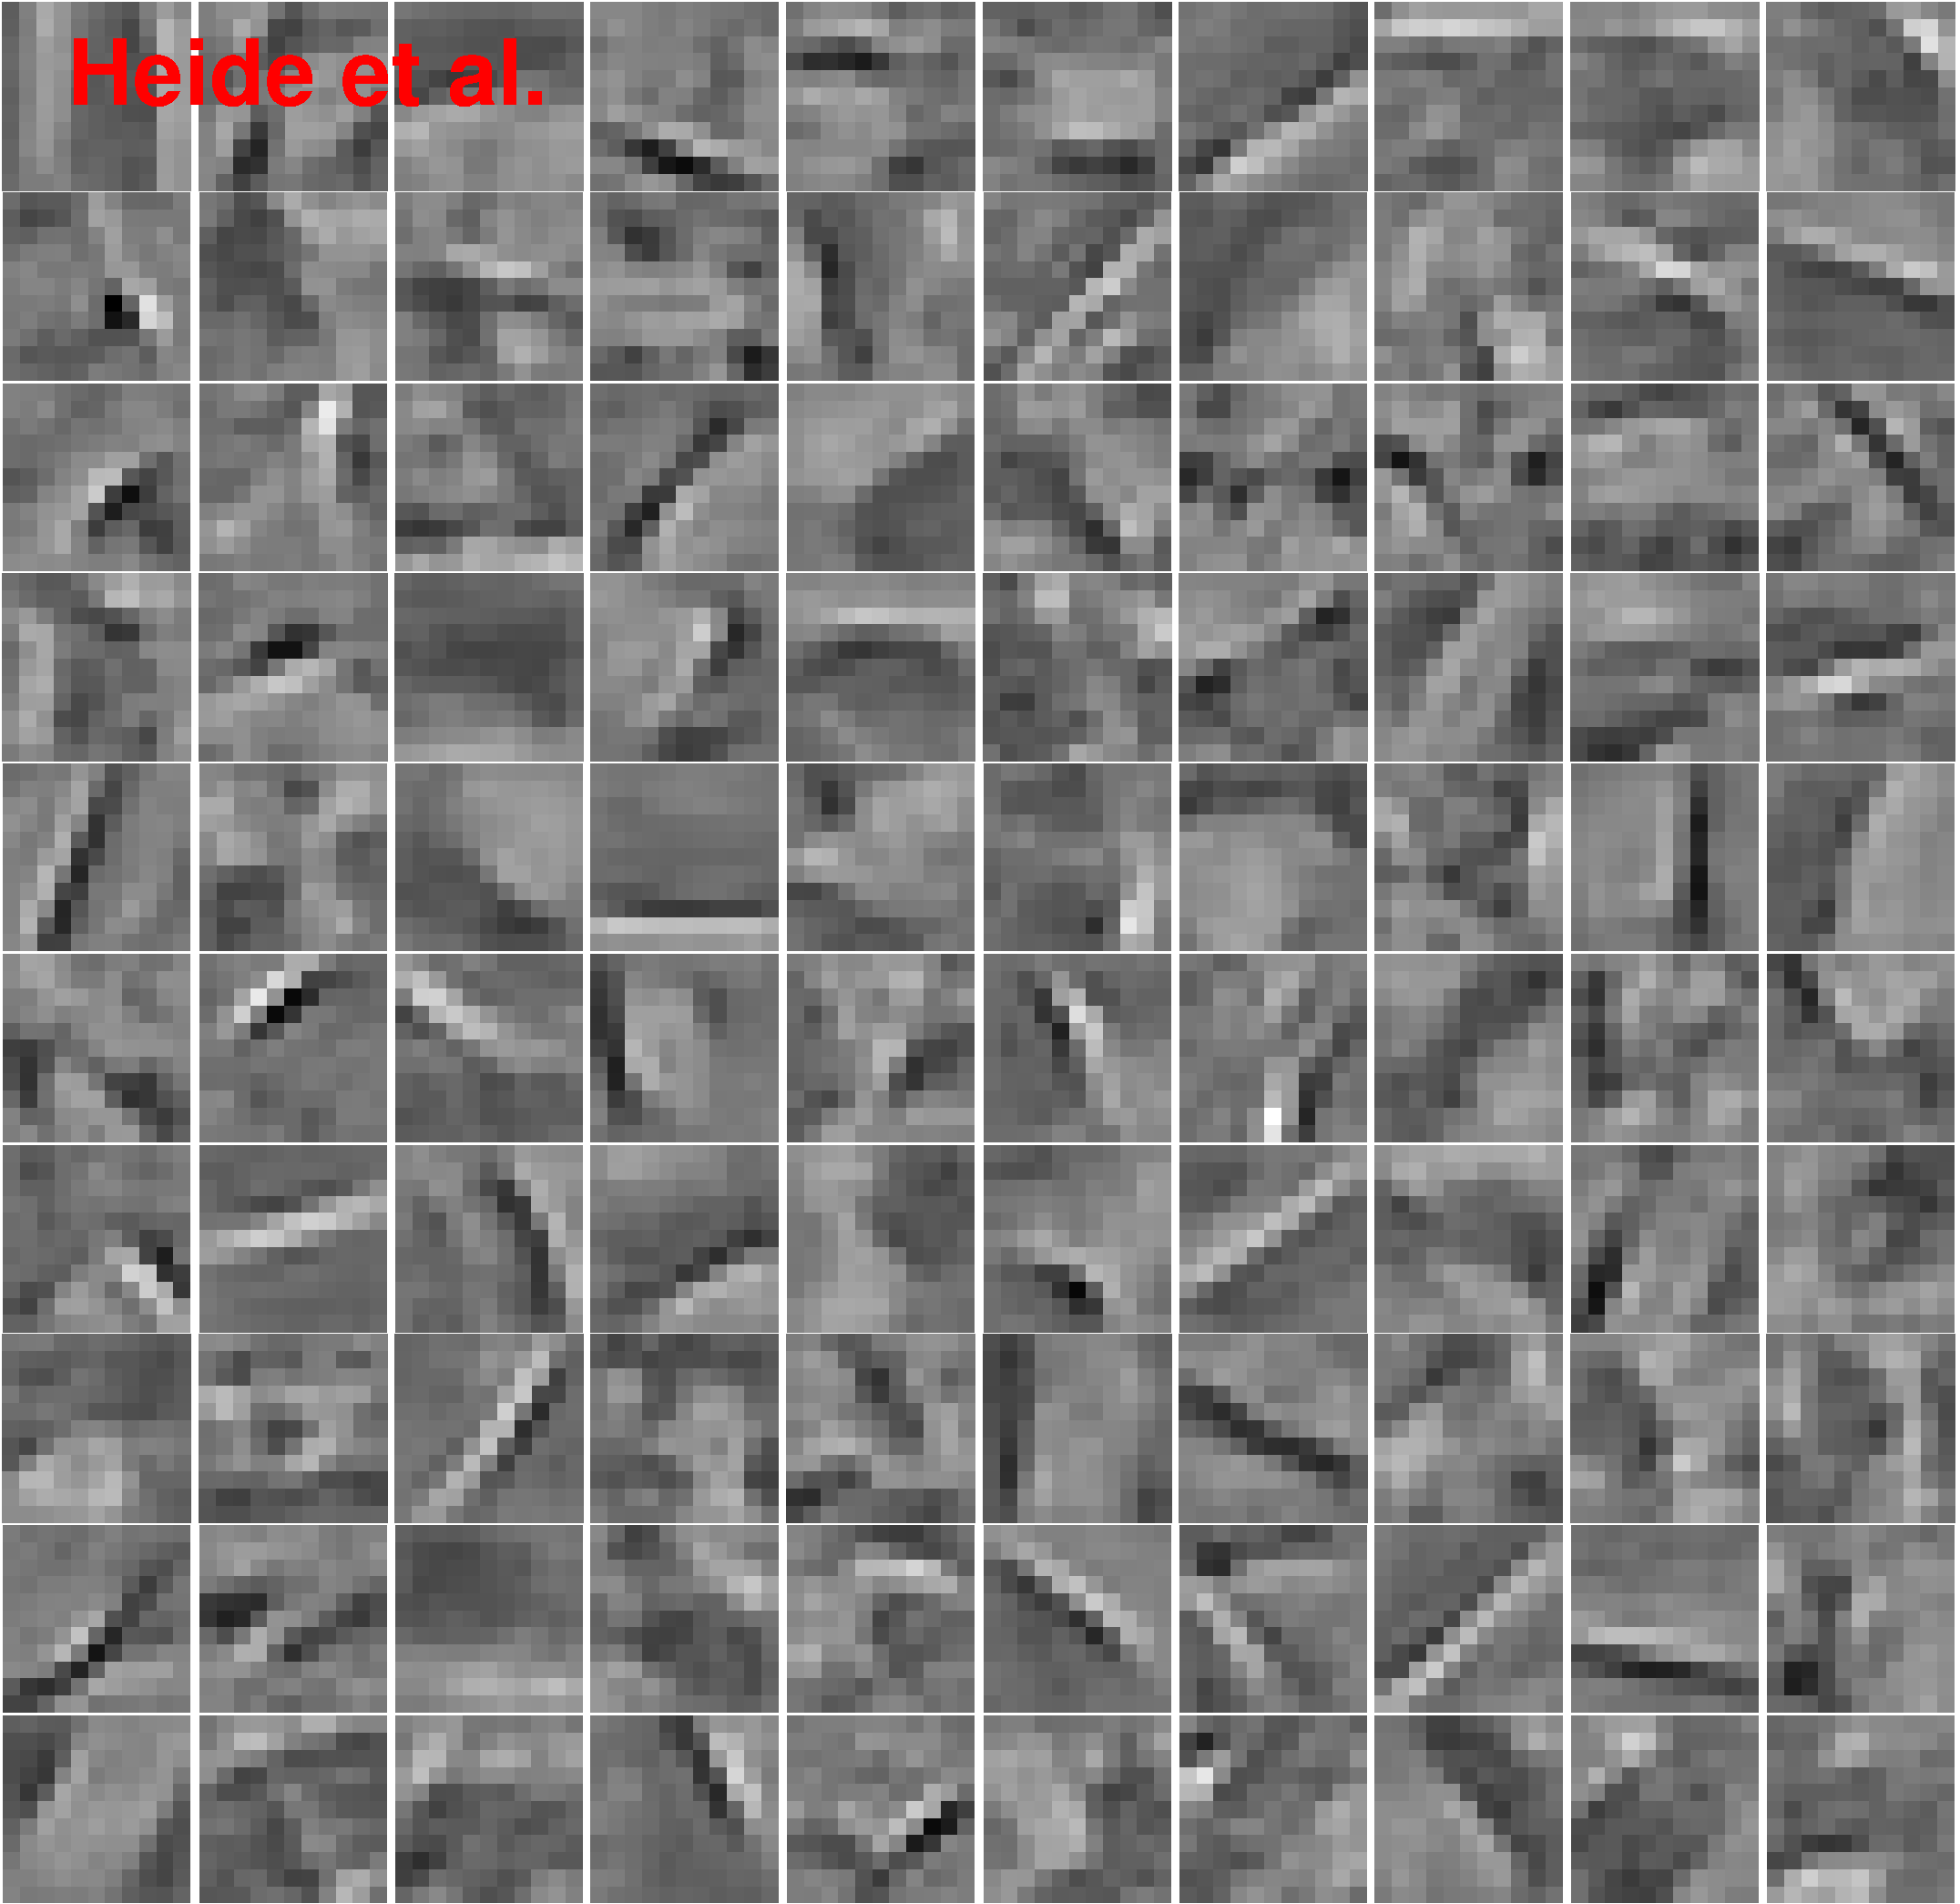
\includegraphics[width=1\linewidth]{figure/heideFruit100.pdf}
\end{subfigure}
\caption{Top: Convergence comparison between the-state-of-art method~\cite{heide2015fast} and the proposed method with different subsampling rate, all of which on performed on fruit dataset. Convergence is evaluated by monitoring the objective value of Eq.~\ref{eq:CSCmodel} on training images versus iterations and time, respectively. Bottom: Learned filters by the proposed method with $p=0.1$ and the comparable method. In these represented learned filters, our method learns more smooth Gabor-like filters and less number of noise-like filters with the same $\lambda$. Beyond this, it runs faster with regard to each iteration and shows better convergence behavior.}
\label{fig:subsampleResult}
\end{figure}

\begin{figure*}[h]
    \centering
    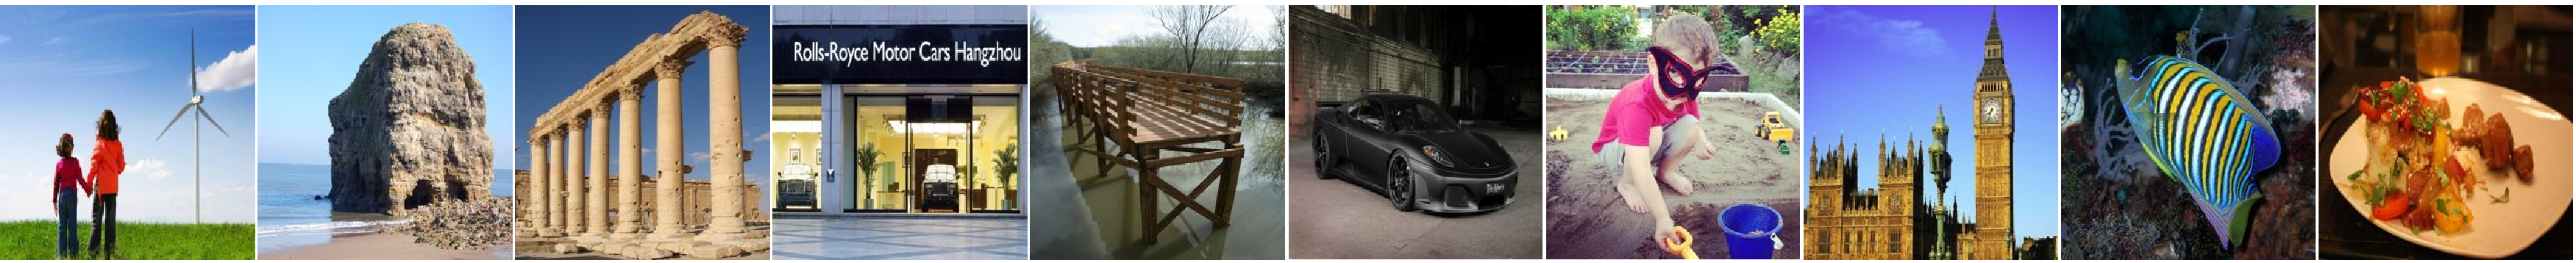
\includegraphics[width=1\textwidth]{figure/reconImage.pdf}
    \resizebox{0.9\linewidth}{!}{
        \begin{tabular}{|c||c|c|c|c|c|c|c|c|c|c|}
            \cline{1-11}
            Image & 1 & 2 & 3 & 4 & 5 & 6 & 7 & 8 & 9 & 10 \\
            \hline
            PSNR~\cite{heide2015fast} & 29.54 & 28.16 & 29.40 & 29.22 & 28.89 & 29.29 & 28.10  & 29.57 & 27.46 & 30.72 \\
            \hline
            PSNR ours & \textbf{29.65} & \textbf{28.18} & \textbf{29.52} & \textbf{29.43} & \textbf{28.99} & \textbf{29.38} & \textbf{28.19} & \textbf{29.63} & \textbf{27.62} & \textbf{30.98} \\
            \hline
        \end{tabular} }
    \caption{Numerical comparisons of the reconstruction quality obtained from the presented filters and its comparison. The reconstructions are performed on $50\%$ randomly observed images, with $\lambda = 0.4$ and $50$ ADMM iterations for both cases. Obtained PSNR values are averaged on 5 trials. Note that none of the testing images are in the training sets.} \label{fig:PSNRrecon}
\end{figure*}

\subsection{Subsampling Strategy}

{\bfseries Convergence.} Comparisons of the convergence between the
proposed method (SBCSC) and the state-of-the-art batch-mode
algorithm~\cite{heide2015fast} are shown in
Fig.~\ref{fig:subsampleResult}. A different selection of the
subsampling rate reveals that the proposed strategy will slightly
influence the convergence and the training objective of the
minimization problem. Specifically, the more subsampled, the
relatively slower convergence and the higher objective will be
obtained. On the other hand, small subsampling rate will significantly
accelerate the computation process, where $10\%$ subsampling achieves
about $6 \times$ speedup over the not subsampled spatial domain solver
and a $2 \times$ speedup over state-of-the-art Fourier-domain solver
for one iteration. We observe that a subsampling rate between $p=0.1$
and $p=0.2$ delivers empirically good enough convergence in our
settings, as well as achieving at least $3 \times$ speedup. In
general, the proposed method with various subsampling rates converges
at around 10-12 iterations in all testing cases, acting similar to the
competing methods.
\note{Not sure what you want to say here -- fix grammar:}
Notice that the comparison method has a relatively
high objective value during the first $6-8$ iterations due to
different splitting strategies are applied and subproblems are
interleaved on the primary variables~\cite{wohlberg2016efficient},
though it converges to an optimum with comparable objective after 10
iterations. In summary, the convergence behaviors of the proposed
algorithm is only slightly influenced by the subsampling strategy
within the testing subsampling rates. Comparing to the
state-of-the-art frequency solver, the proposed stochastic
spatial-domain solver with a subsampling rate of $0.1$ reduces the
computation time by a factor of two for the tested example. The
robustness of the proposed algorithm is evaluated by additional
experiments. Please see supplementary materials for reference.

{\bfseries Reconstruction}. The SBCSC-learned filters with a
subsampling rate of $p=0.1$ are shown in the bottom of
Fig.~\ref{fig:subsampleResult}. For a visual comparison, we also show
the filters learned from the competing method (bottom left of Figure 3
in~\cite{heide2015fast}). As can be observed, both of them learn some
seemingly similar Gabor-like filters. However, zooming into the
details (please see supplemental materials for high resolution
versions) reveals that our filters appear less noisy than the ones
from~\cite{heide2015fast}. We then demonstrate the effectiveness of
the reconstructed filters in the application of image inpainting,
which refers to reconstructing a full image from partial
measurements. A numerical comparison of the reconstruction quality is
shown in Fig.~\ref{fig:PSNRrecon}. The filters learned by the proposed
method not only appear less noisy by themselves, but also achieve
better reconstruction quality on partially observed images with
respect to the PSNR value. Furthermore, the learning process
only takes about $50\%$ of the time for our method. Specifically, SBCSC takes 170 seconds and the comparable method takes 350 seconds for 14 iterations on a Core i7 PC.

\subsection{Online Learning}

{\bfseries Convergence.} Unlike the batch-based learning approaches
which evaluate its convergence by monitoring the objective value on
training datasets, a common way to evaluate the learning process of
online learning model is to monitor its objective value on test
datasets. In Fig.~\ref{fig:onlineSmall} we plot the objective values
against the iteration number for the proposed method (SOCSC) and a
recent online frequency-domain CSC method~\cite{liu-2018-first}. In
the same figure, we also keep track of the capability of the updated
filters during the learning process to sparsely represent the test
images, which is demonstrated by the time evolution of PSNR. These two
approaches stop at optimum positions with similar objective values.
%although they exhibit slightly different convergence behaviors with
%respect to iterations.
The final PSNR values for both methods also reveal a similar
reconstruction performance of the learned filters. In terms of runtime
comparison, however, the proposed method runs at least $6$ times faster
than the comparison method. Specifically, SOCSC takes 70 seconds and the comparable method takes 440 seconds on a Core i7 PC to process all 10 training images. The supplement shows additional comparisons for the other datasets.

%The proposed method not only exhibits a better convergence performance, but also takes much less execution time, achieving roughly $5 \times$ speedup for one iteration. A visual comparison of the learned dictionaries also demonstrates that the proposed algorithm delivers better outcomes.
% Further numerical comparison will be reported in the next section.

{\bfseries Over-complete dictionary.} To our knowledge, none of the
existing CSC work reported or analyzed the over-complete dictionary
(number of the dictionary is more than its degrees of freedom). One of
the reasons could be that most of the prior work is batch-based, thus
learning over-complete dictionary from small datasets would cause
overfitting issues, which may contain quite a few data-specific
filters, and therefore limit the ability to generalize the filters to
other data (we verify this explanation in the supplement). The
proposed online-based learning strategy (SOCSC) can overcome this
issue by scaling the model up to arbitrary sample sizes.

\begin{figure}[h]
\centering
\begin{subfigure}{0.49\textwidth}
  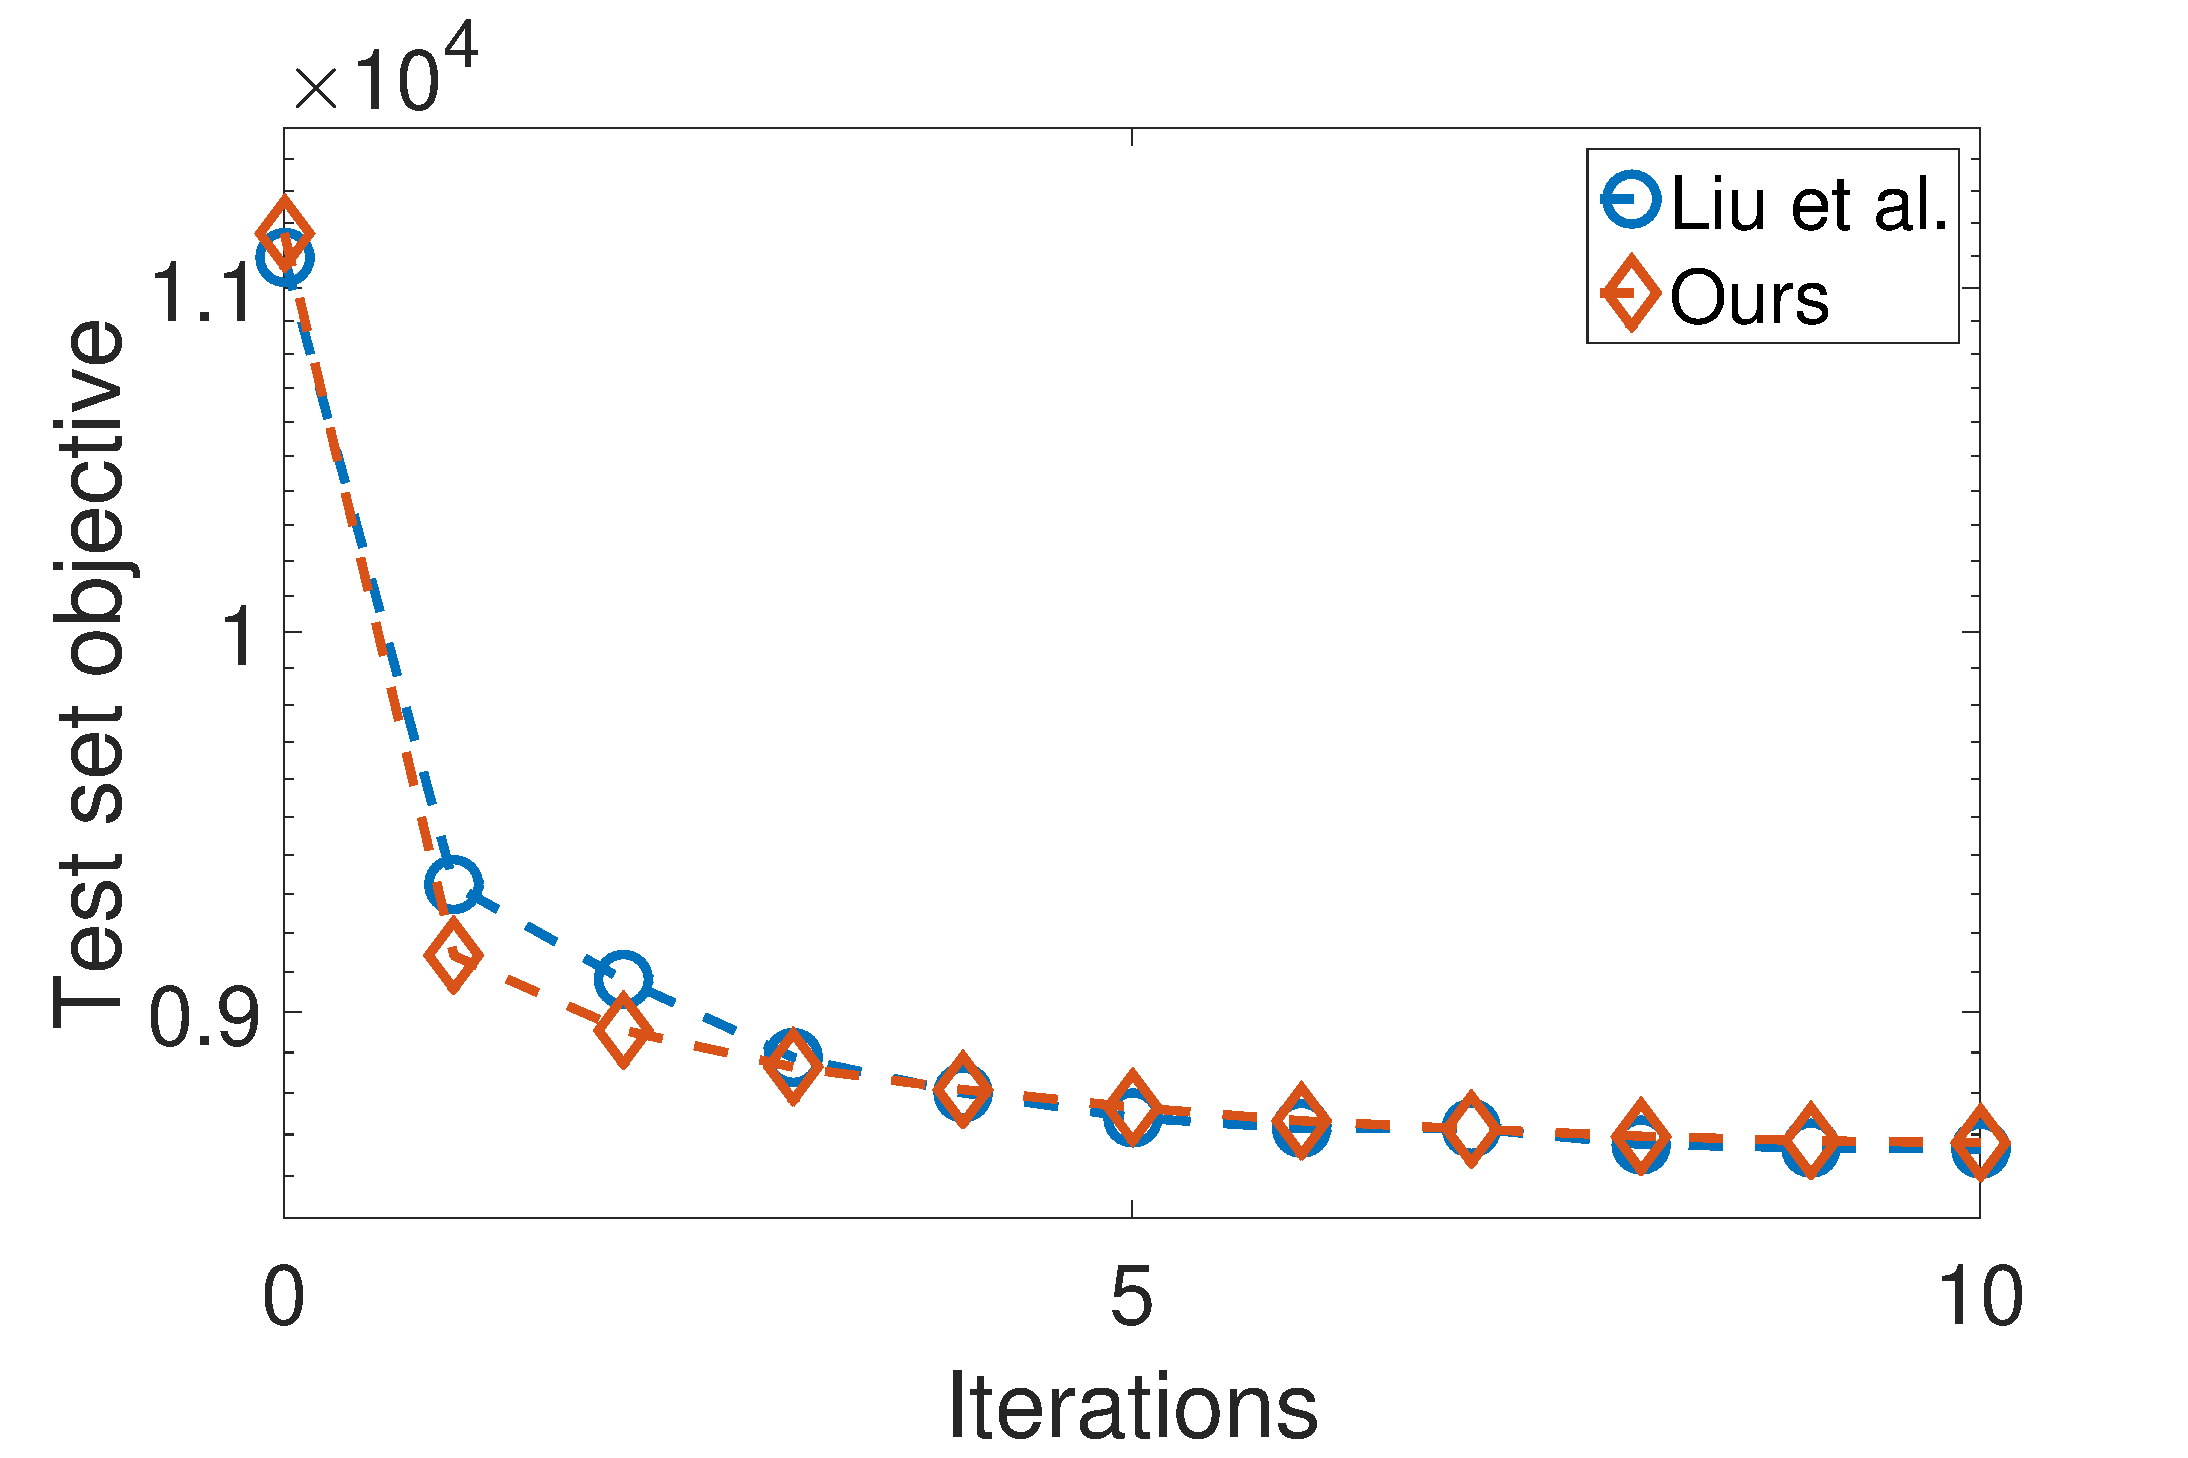
\includegraphics[width=1\linewidth]{figure/onlineVSliu-ite-fruit.pdf}
\end{subfigure}
\begin{subfigure}{0.49\textwidth}
  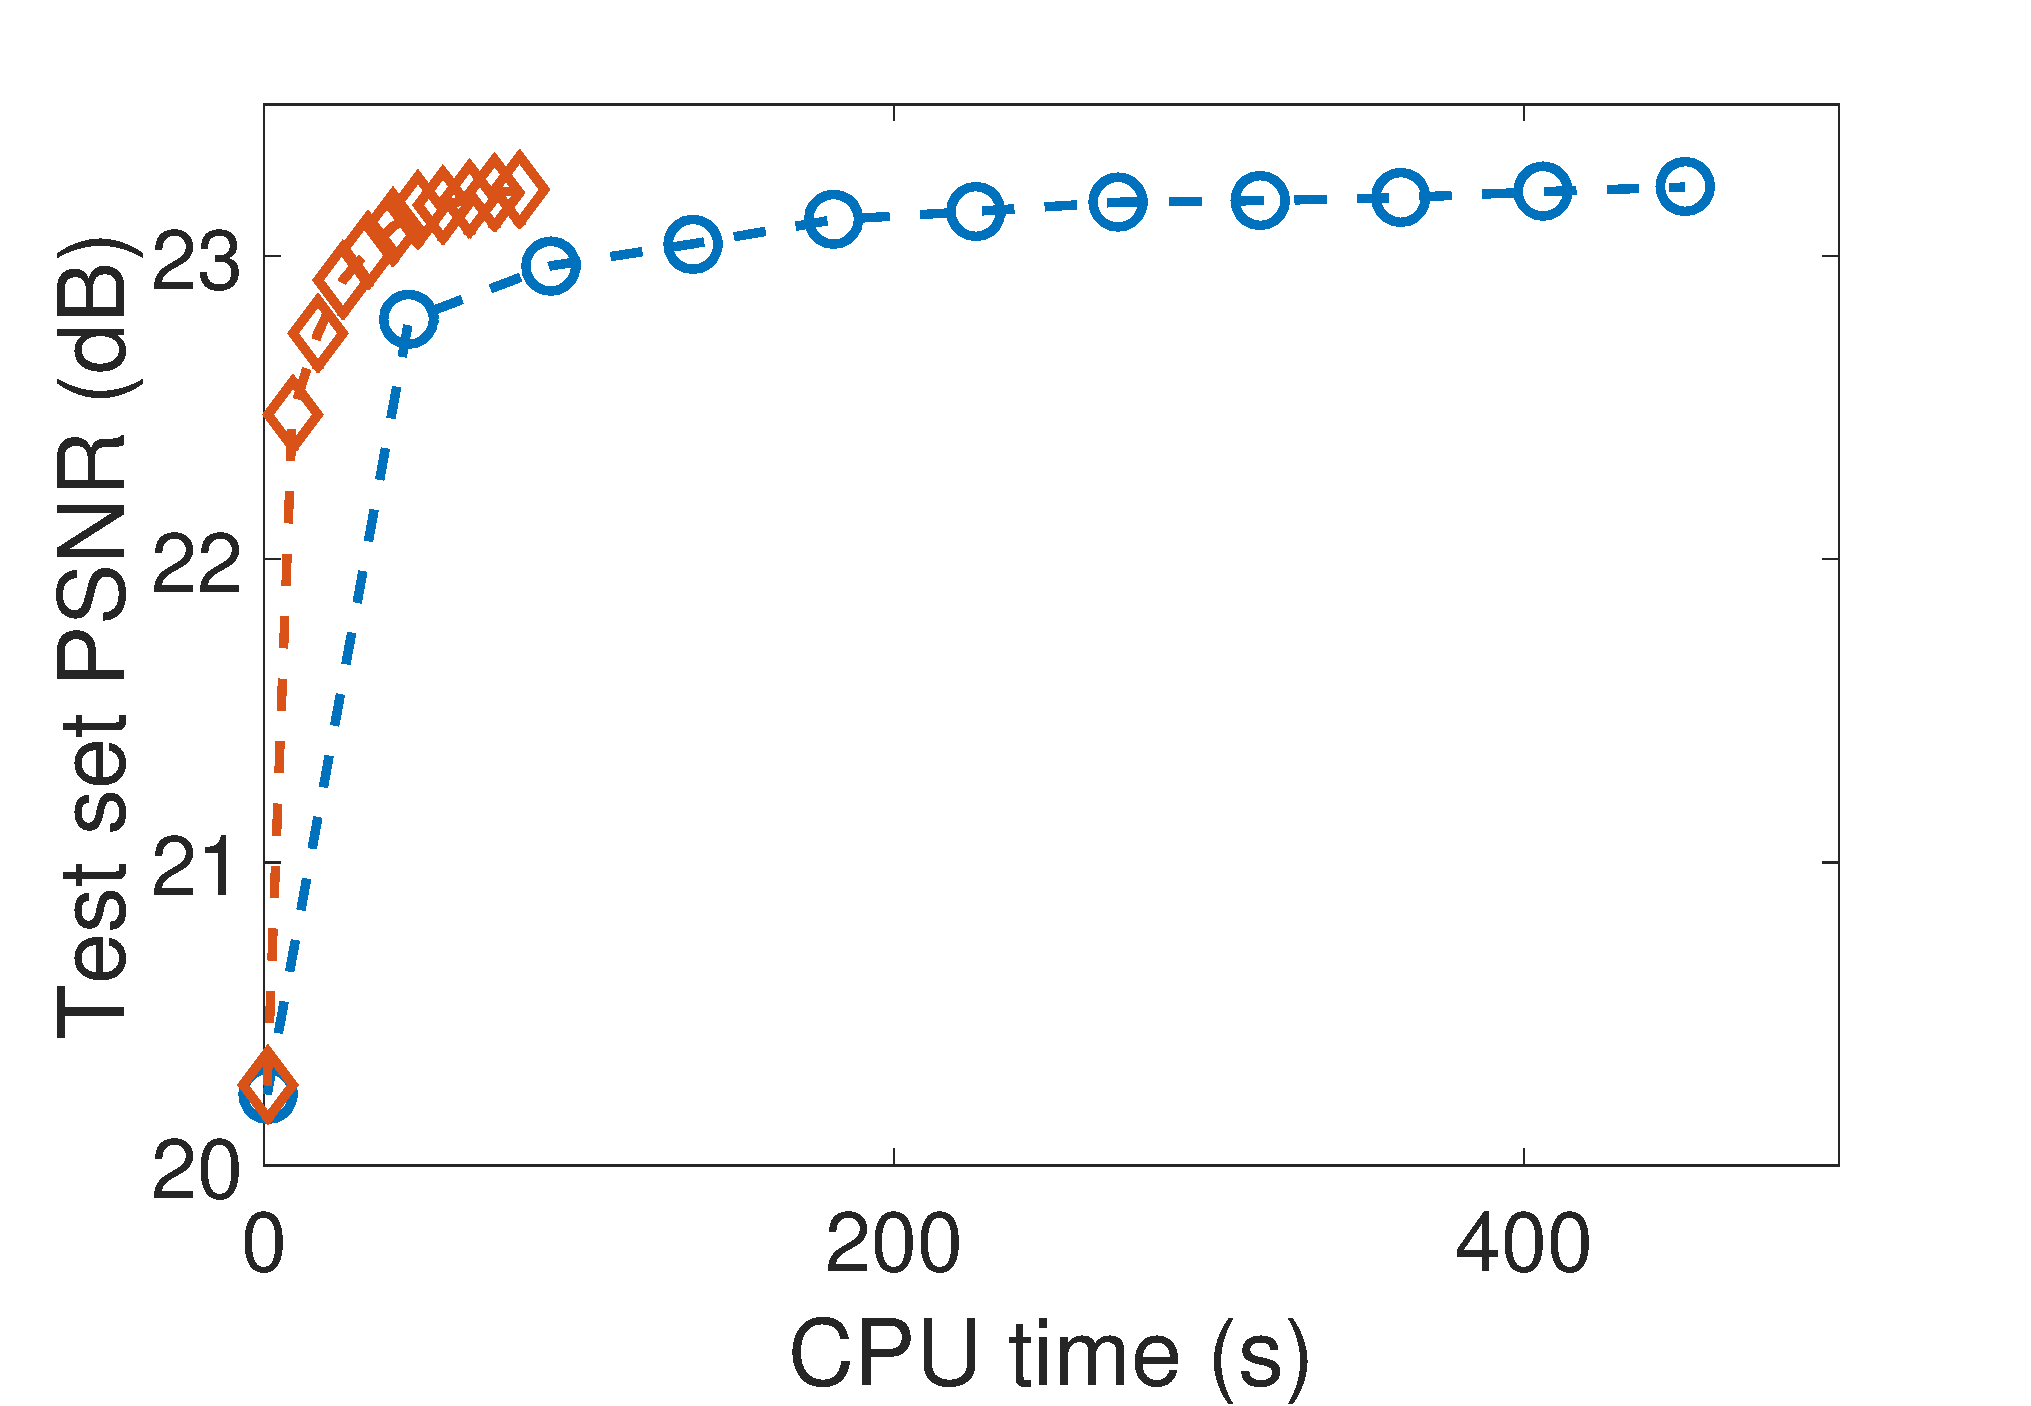
\includegraphics[width=1\linewidth]{figure/onlineVSliu-time-fruit.pdf}
\end{subfigure}

\caption{The experiments are performed on fruit dataset, and each iteration randomly choose one samples from the training datasets. Top: Convergence of the test set objectives (objective value of Eq.~\ref{eq:CSCmodel} on testing datasets) for our method (SOCSC) and the state-of-the-art online approach~\cite{liu-2018-first}. Bottom: Testing PSNR with respect to execution time. While the quality of the output is comparable, our method achieves $6 \times$ speedup.}
\label{fig:onlineSmall}
\end{figure}

\begin{figure*}[h]
\begin{minipage}{0.4\textwidth}
\begin{subfigure}{1\textwidth}
    \centering
  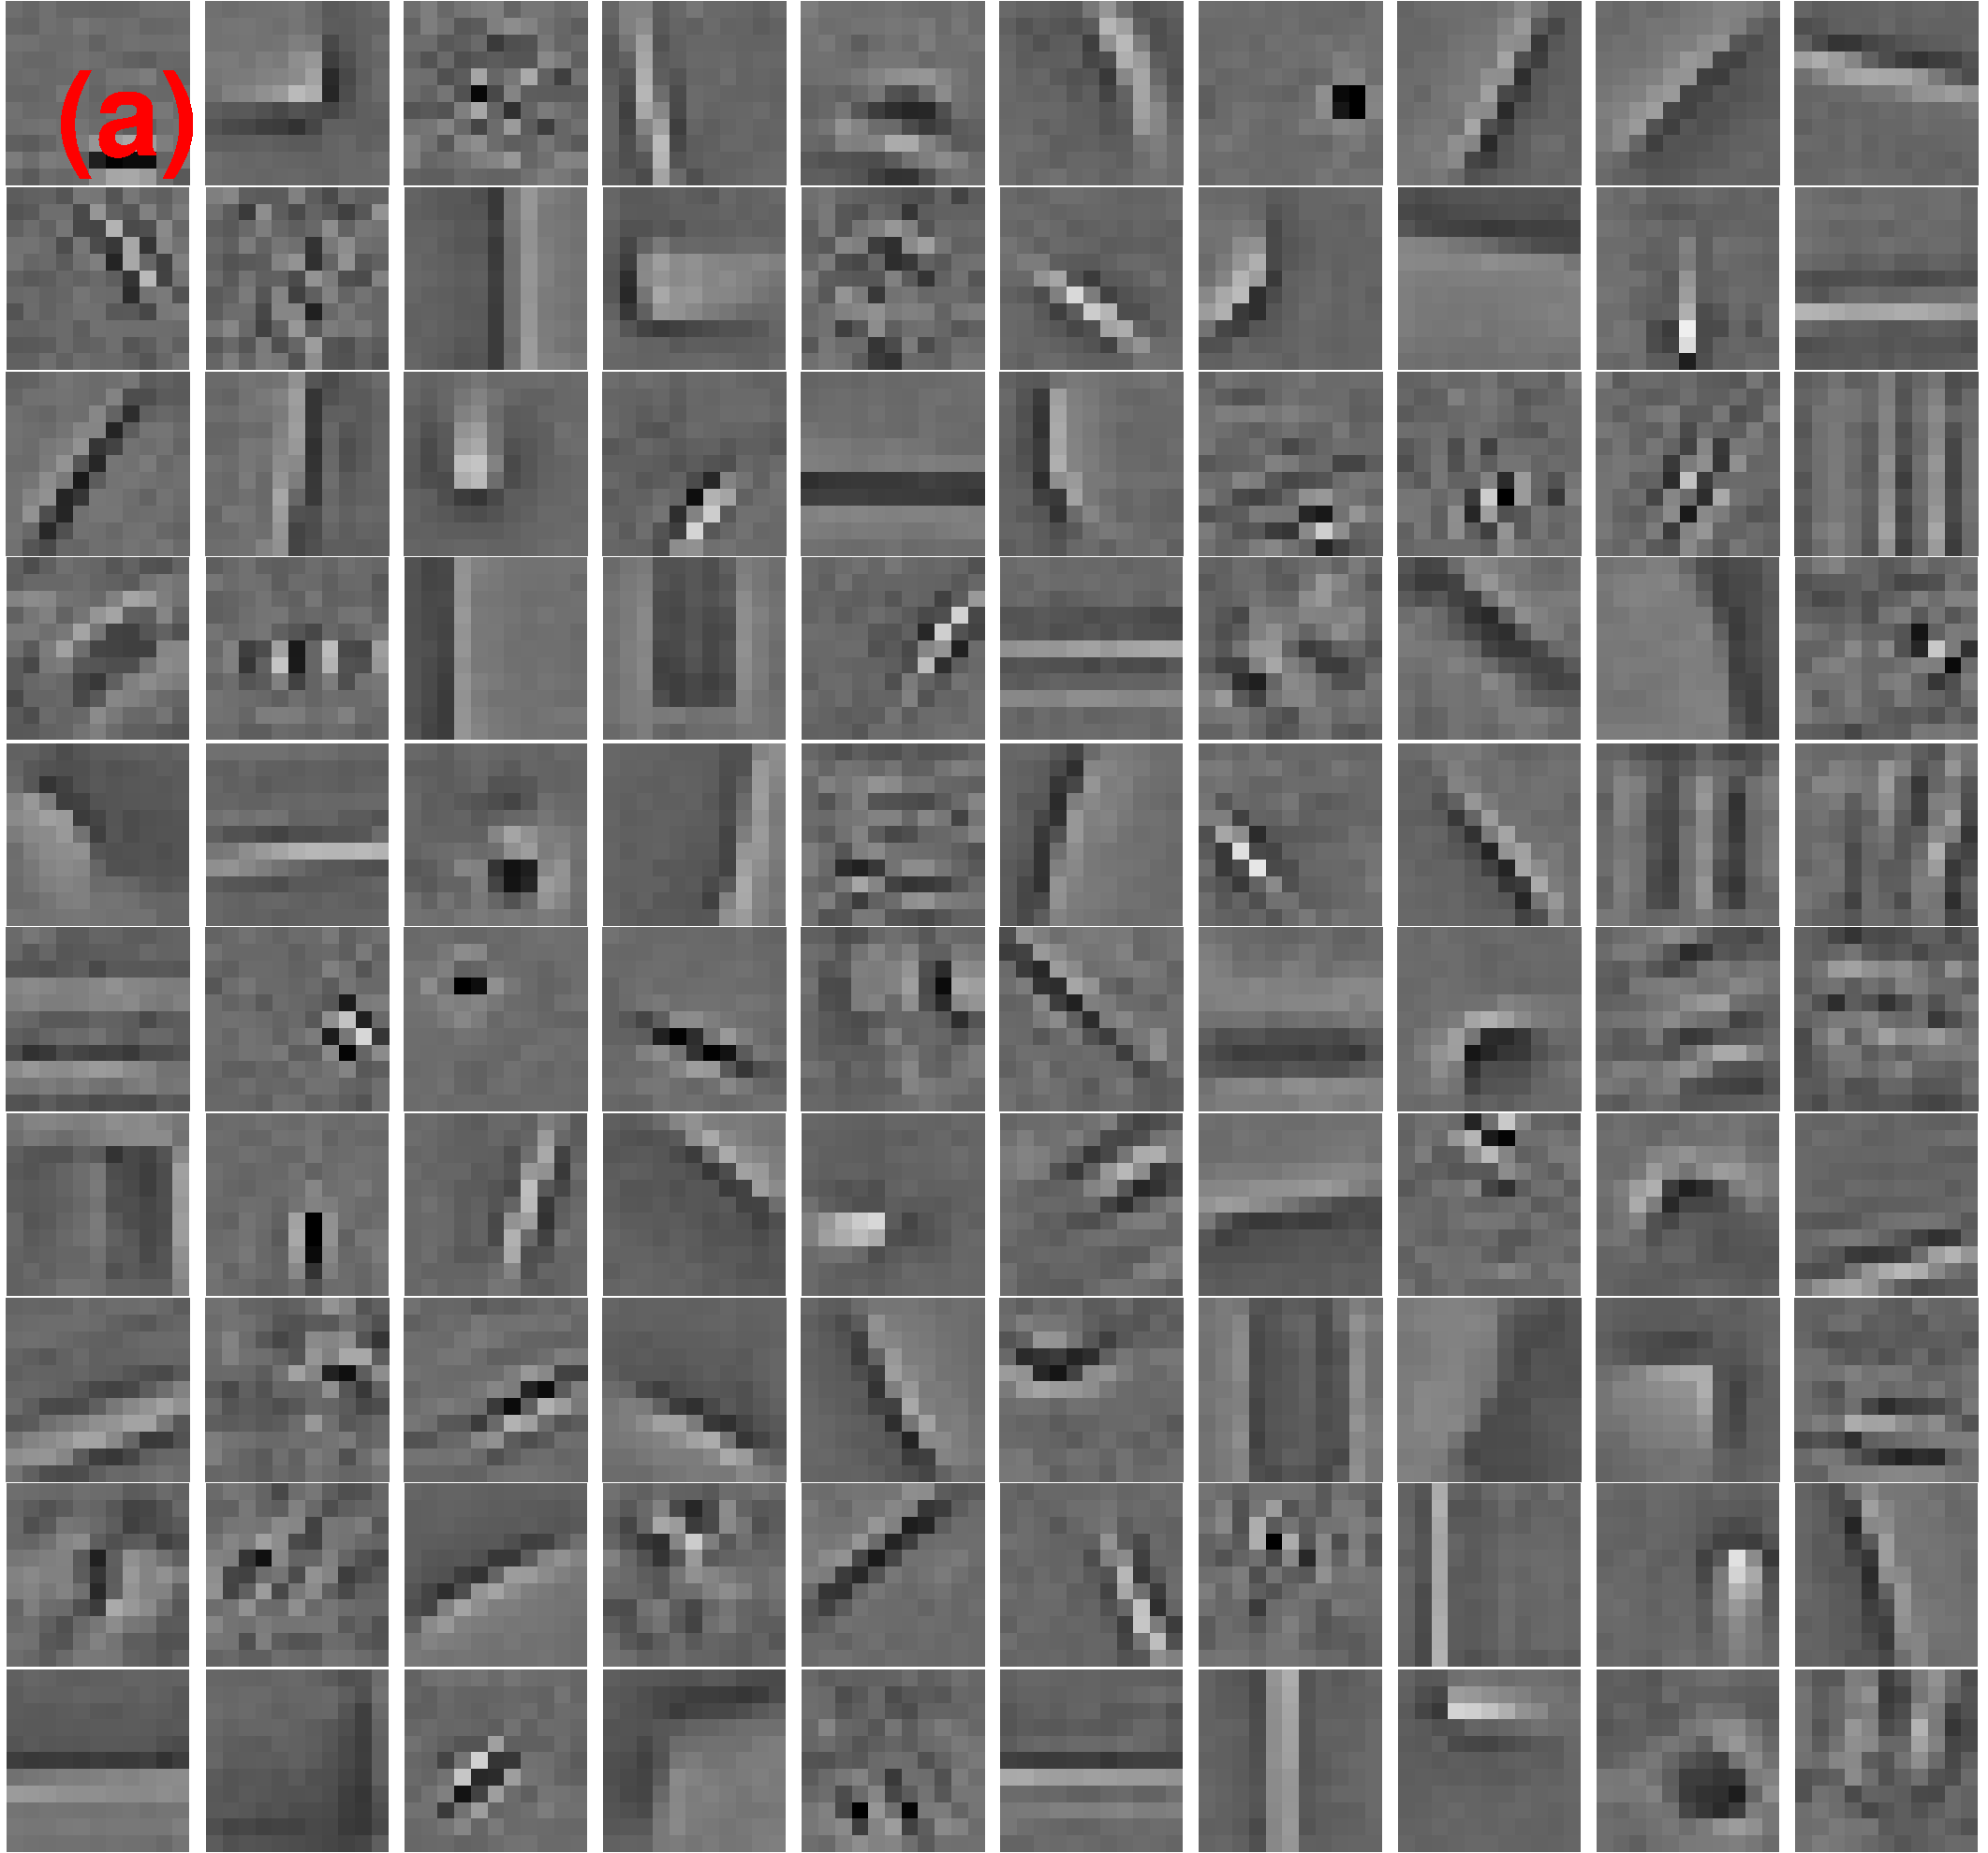
\includegraphics[width=0.75\linewidth]{figure/liu100-filter.pdf}
  \vspace*{2mm}
\end{subfigure}

\begin{subfigure}{1\textwidth}
    \centering
  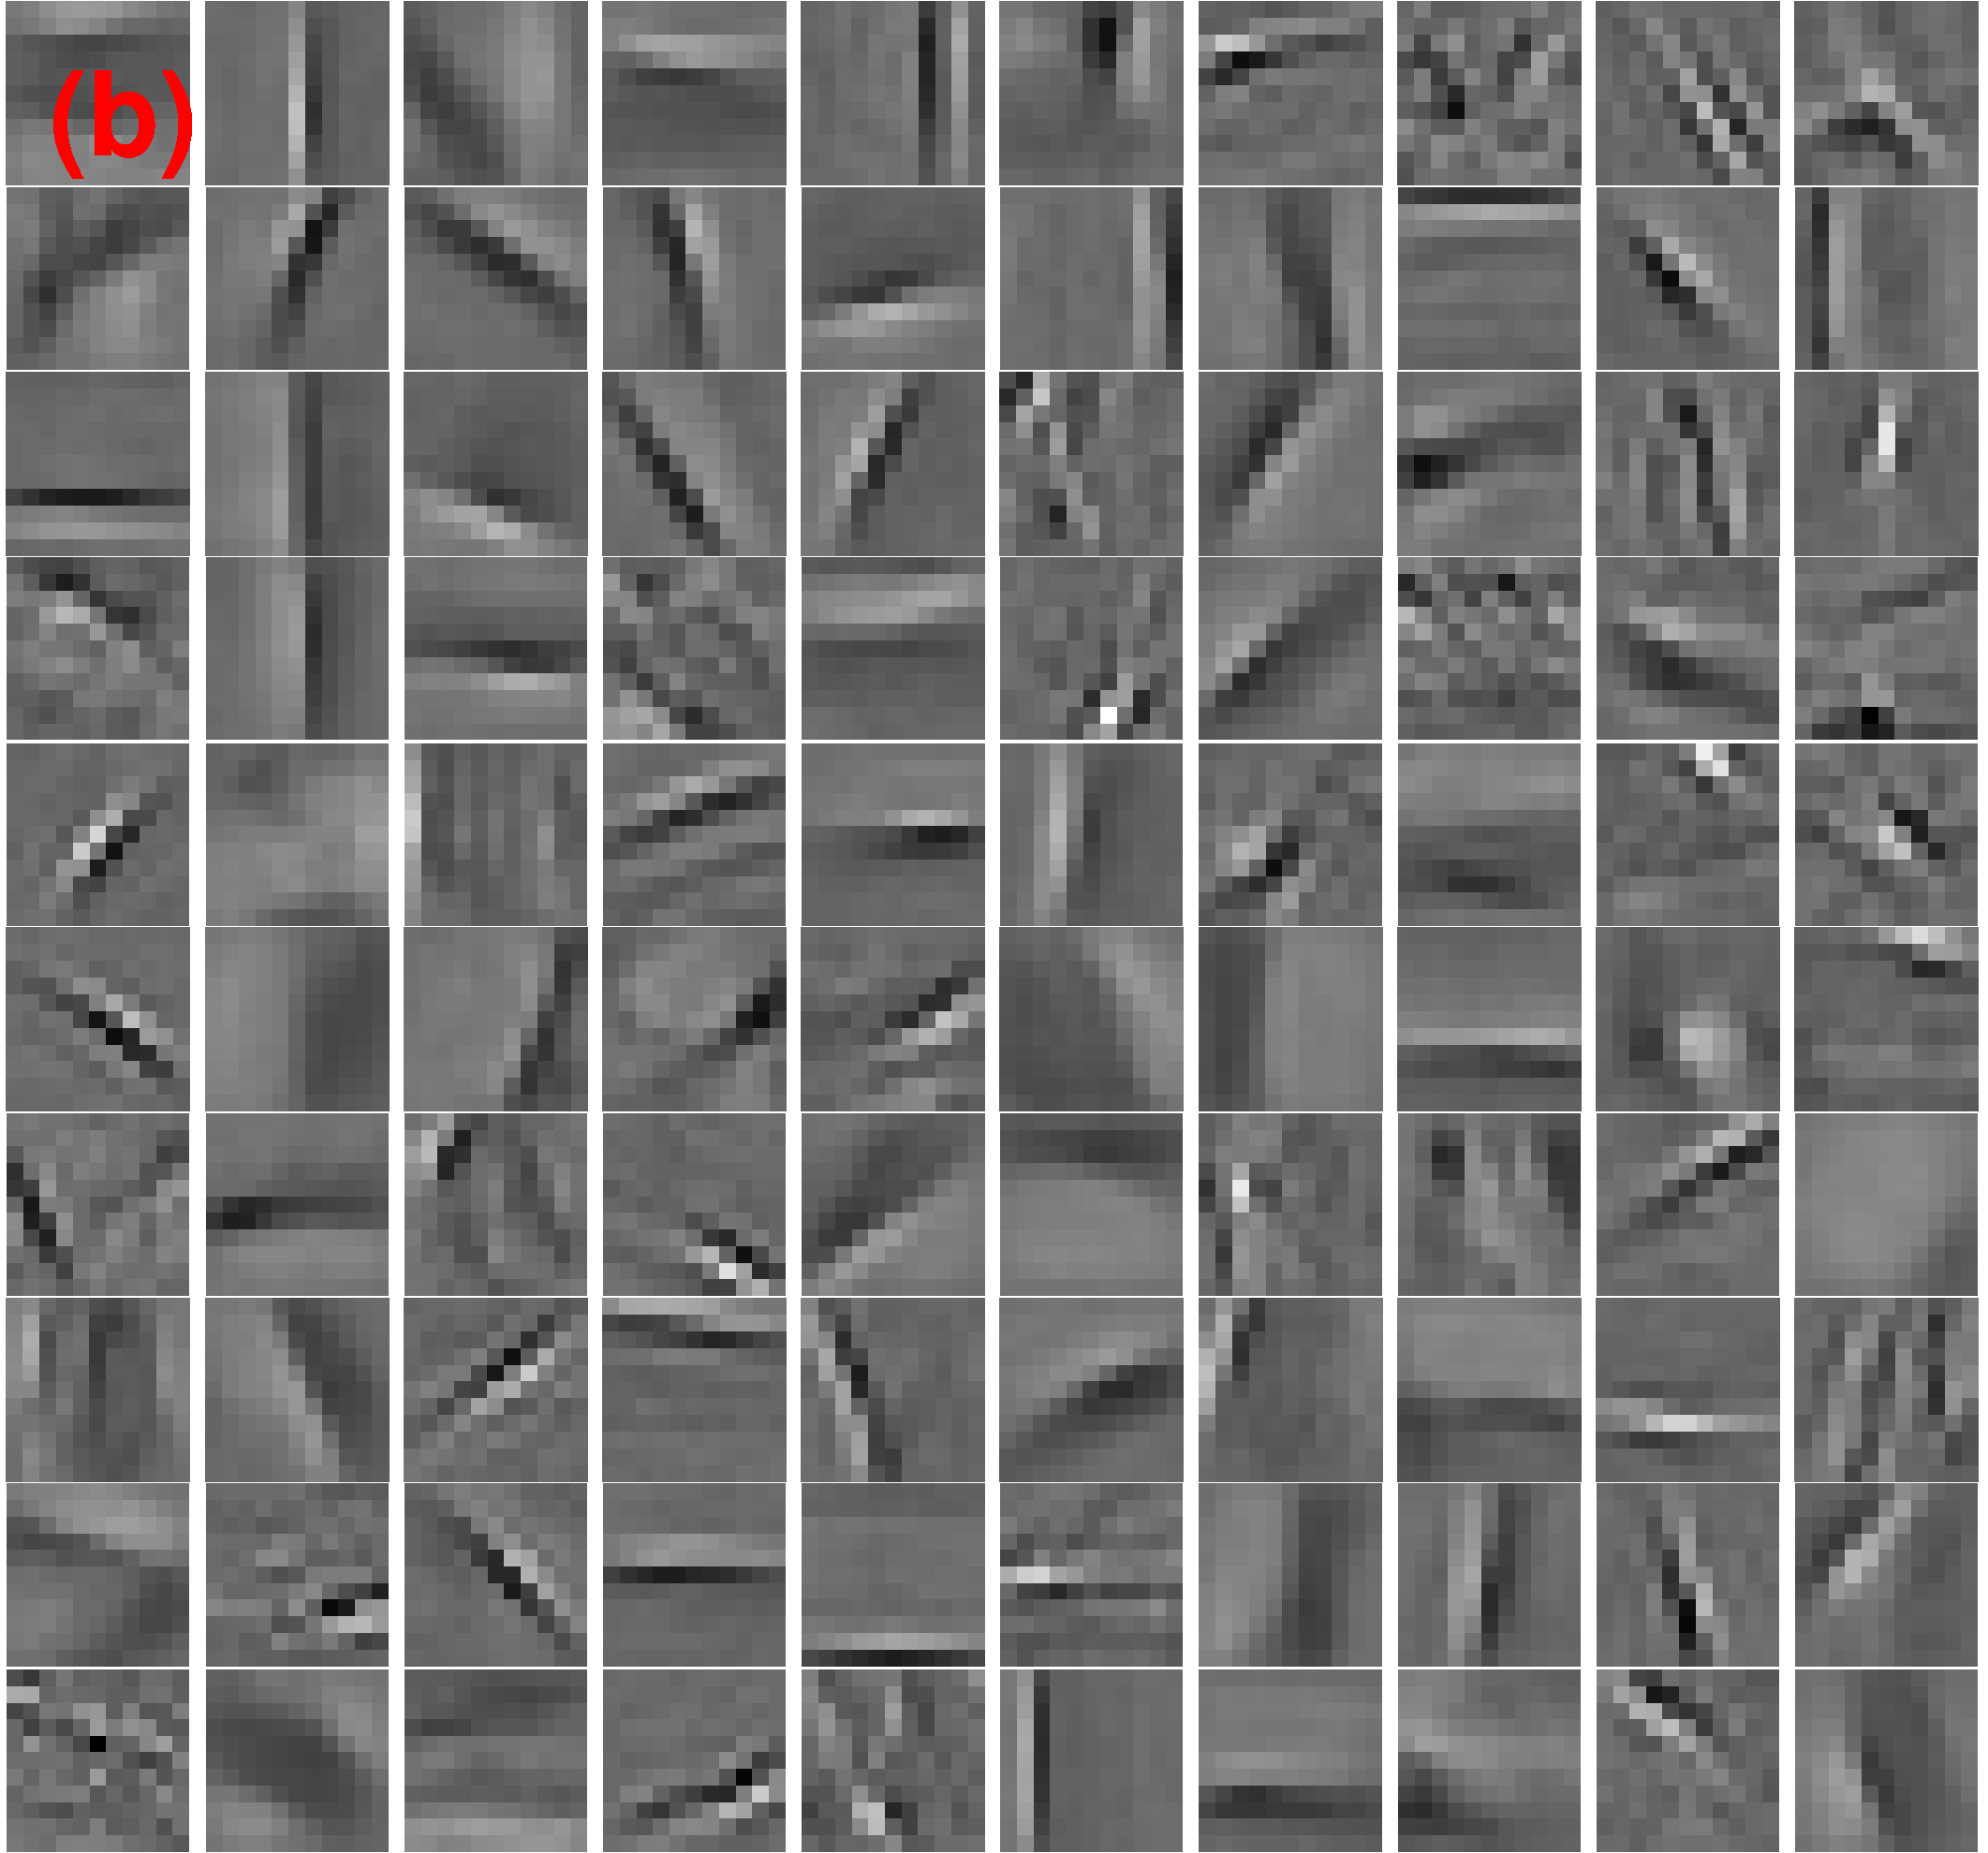
\includegraphics[width=0.75\linewidth]{figure/online100-filter.pdf}
\end{subfigure}
\end{minipage}
\begin{minipage}{0.6\textwidth}
\centering
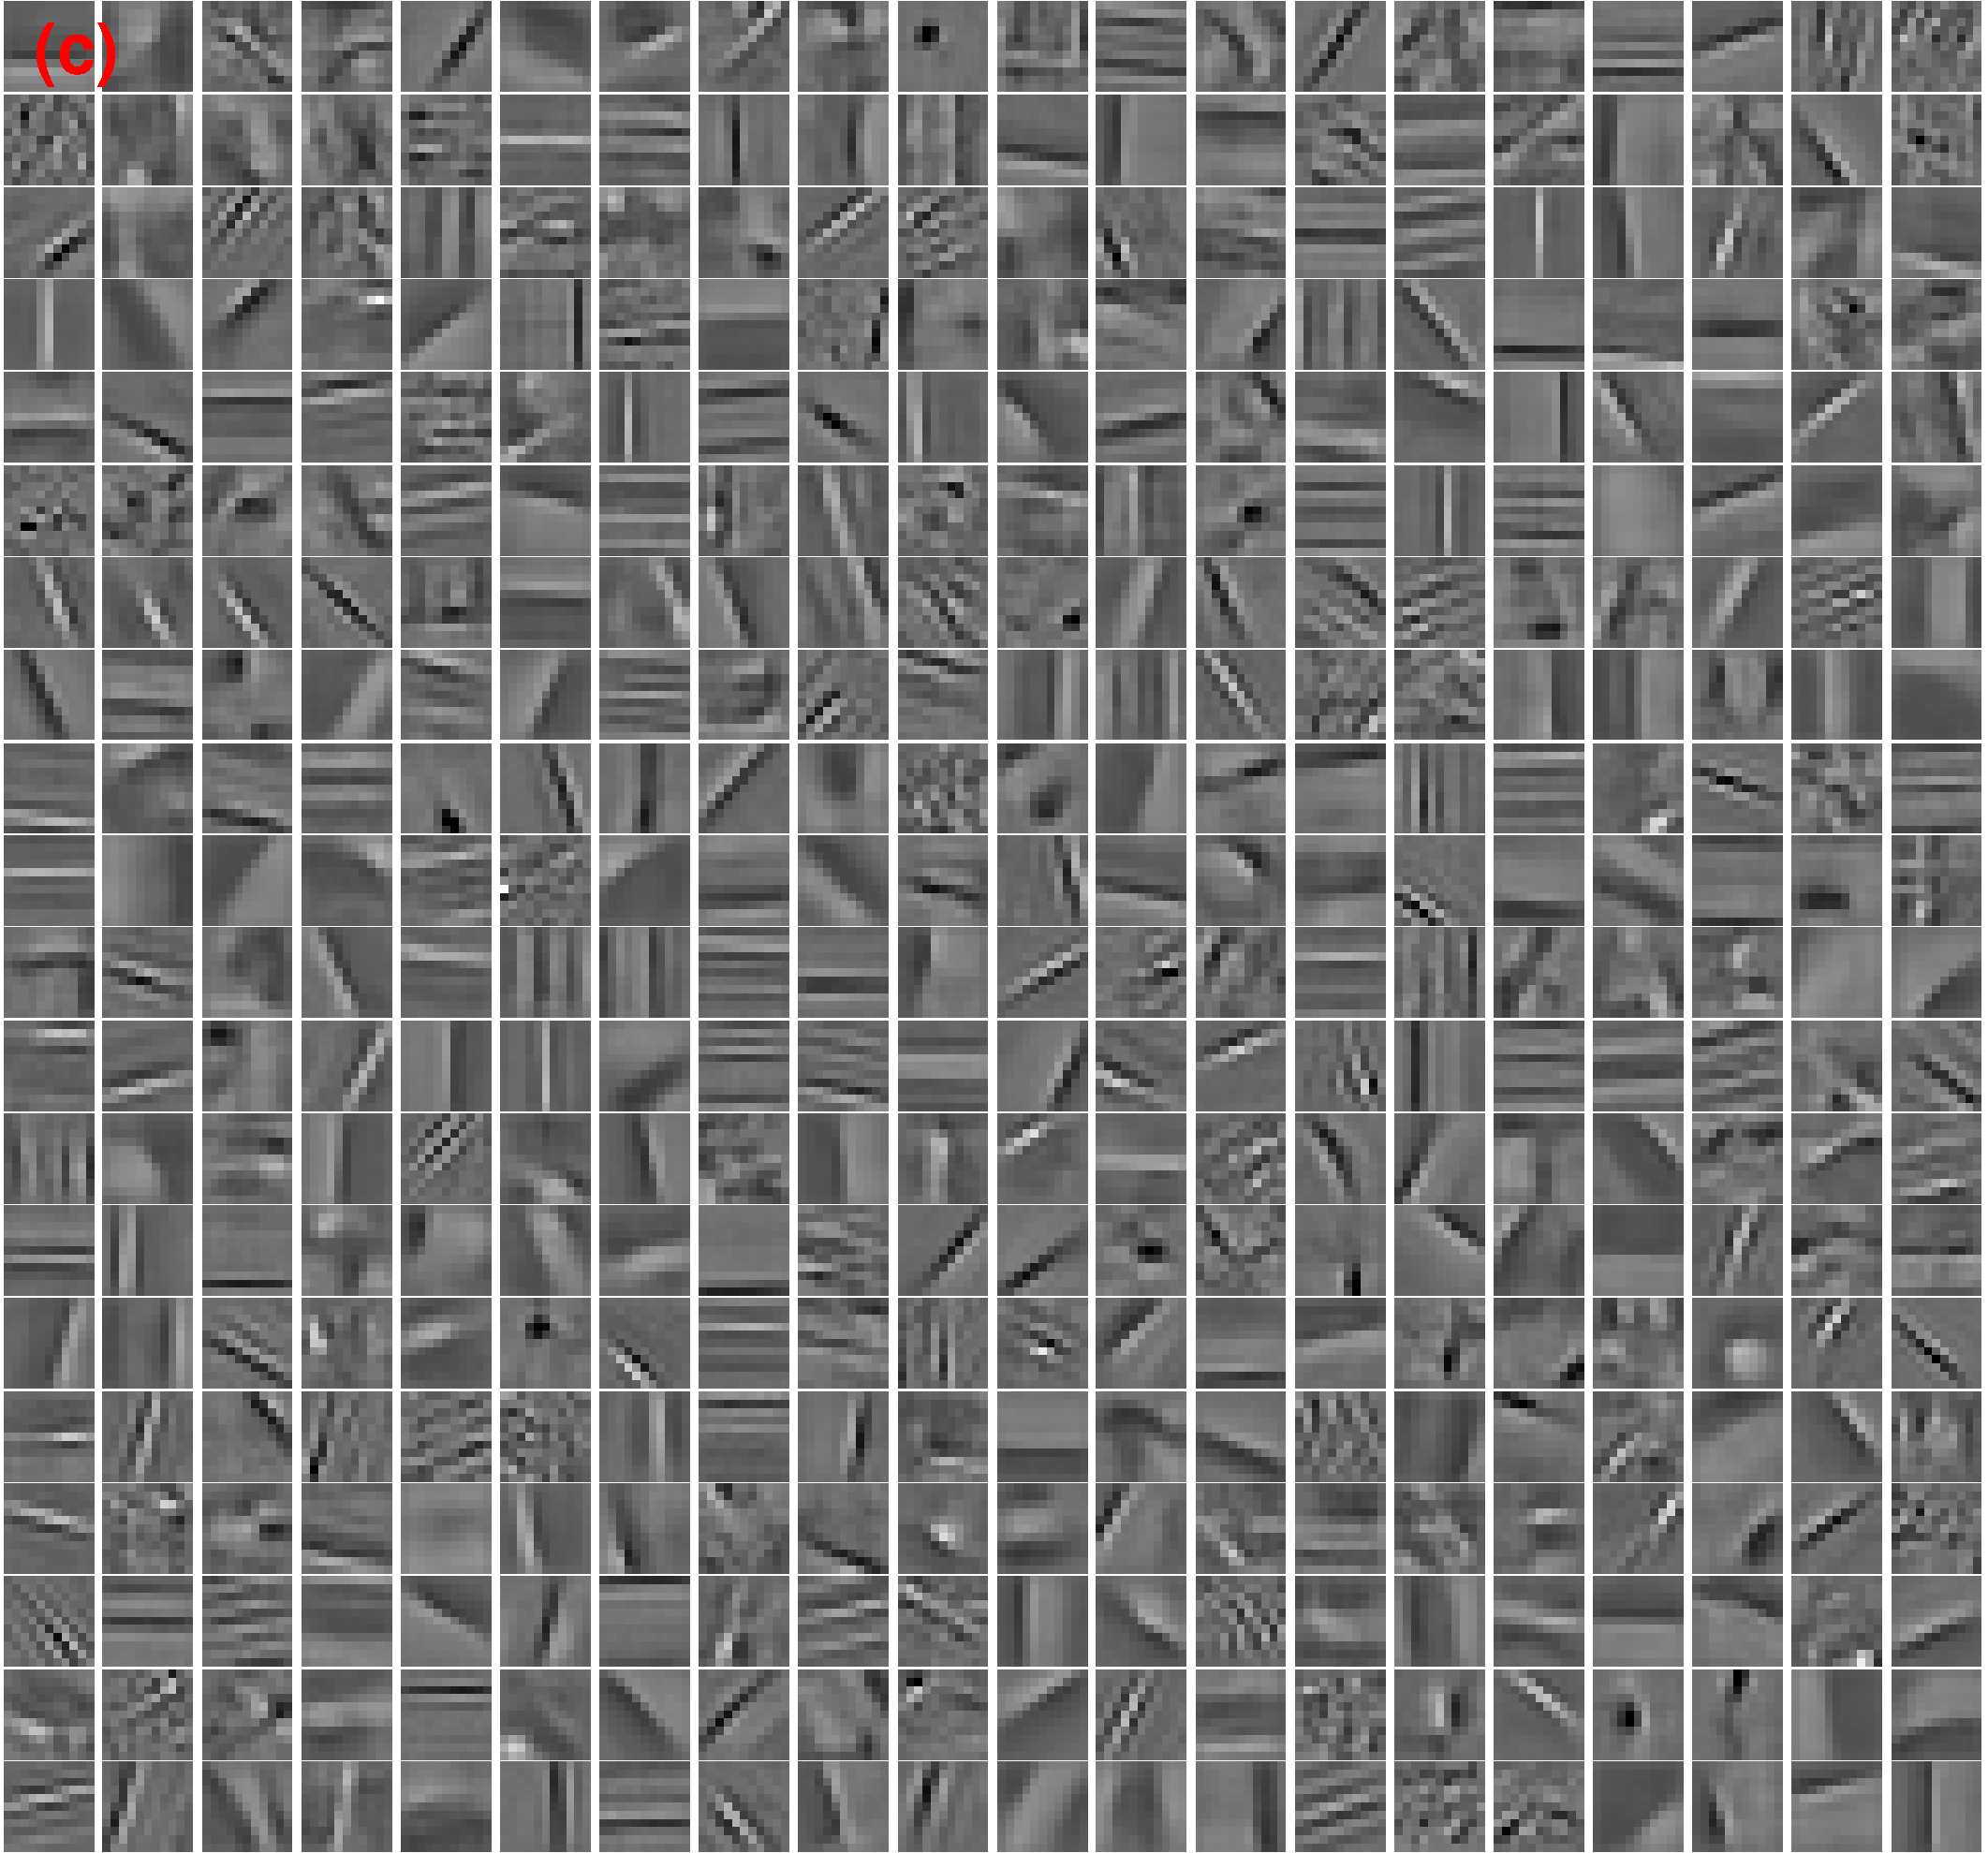
\includegraphics[width=0.97\linewidth]{figure/online400-filter.pdf}
\vspace*{2mm}
\end{minipage}
\begin{minipage}{1\textwidth}
    \centering
    \resizebox{0.8\linewidth}{!}{
        \begin{tabular}{|c||c|c|c|c|c|c|c|c|c|c|}
            \cline{1-11}
            Image & 1 & 2 & 3 & 4 & 5 & 6 & 7 & 8 & 9 & 10 \\
            \hline
            PSNR by (a) & 29.58 & 28.19 & 29.44 & 29.63 & 28.89 & 29.33 & 28.13  & 30.14 & 27.42 & 30.89 \\
            \hline
            PSNR by (b) & 29.63 & 28.22 & 29.57 & 29.90 & 29.12 & 29.59 & 28.05  & 30.17 & 27.53 & 31.08 \\
            \hline
            PSNR by (c) & \textbf{30.24} & \textbf{28.34} & \textbf{29.95}  & \textbf{30.30} & \textbf{29.43} & \textbf{29.96} & \textbf{28.24} & \textbf{30.57} & \textbf{27.72} & \textbf{31.67} \\
            \hline
        \end{tabular} }
\end{minipage}
\caption{Filters learned from 1000 images by our method (SOCSC) and the state-of-the-art online method~\cite{liu-2018-first}, and their corresponding reconstruction quality using the same hyperparameter settings as in Fig.~\ref{fig:PSNRrecon}. (a) The under-complete dictionary ($11 \times 11 \times 100$) learned by~\cite{liu-2018-first}; (b) The under-complete dictionary ($11 \times 11 \times 100$) learned by SOCSC. (c) The over-complete dictionary ($11 \times 11 \times 400$) learned by SOCSC. These under-complete dictionaries, mainly composed of Gabor-like filters, can be seen as a subset of the represented over-complete dictionary, which contains a number of extra low contrast image features.}
\label{fig:overCompleteDic}
\end{figure*}

We demonstrate this ability on 1000 image patches with the size of
$100 \times 100$, and learn an $11 \times 11 \times 400$ over-complete
dictionary, which is shown in Fig.~\ref{fig:overCompleteDic}. For a
visual comparison, we also show $100$ learned filters generated by the
same algorithm and another 100 filters generated
by~\cite{liu-2018-first}. As can be observed, both of the approaches
learn visually similar under-complete dictionary, while the proposed
method takes $6 \times$ less training time than the comparison
method. The learned over-complete dictionary is composed of
the Gabor-like image features as represented in the under-complete
dictionaries, as well as a number of low contrast features which are
not typical for under-complete dictionaries. This additional
feature information would play an essential role to better reconstruct
the natural images, which can be demonstrated by the results of
reconstruction quality shown at the bottom of the same figure.

We further show a bottleneck revealed by the under-complete dictionary
in the online-based CSC model. The top of
Fig.~\ref{fig:overComDicAndMinibatch} demonstrates that no more
apparent progress could be observed when the number of training images
is higher than a specific value for both of the online approaches
($K=100$). However, owing to more abundant filters, learning
over-complete dictionary overcomes this bottleneck, and it shows a
considerable improvement in the PSNR of image representations.  This
is also verified by applying these learned dictionaries to the image
inpainting application as discussed above.

{\bfseries Mini-batching.} In practice, a mini-batching strategy would
be preferred in order to gain advantages from modern parallel
computing architectures. This is also a standard extension to
stochastic optimization algorithms~\cite{Takac2013, PCDM, SCSG}. We
denote the mini-batch size as $\eta$. In the proposed online algorithm
(SOCSC), the time complexity for one step dictionary update will not
increase linearly with the increase of $\eta$. Concretely speaking,
updating $\code$ can be implemented by caching the Cholesky
decomposition, and one computation of the matrix factorization can be
applied to all of the currently selected batches. Herein, the
complexity for doing updating $\code$ $\eta$ times all together is
cheaper than $\eta$ times the complexity of updating one $\code$. In
addition, the time complexity for updating $\filter$ is not linearly
affected by the value of $\eta$, which will be executed only once in
each training step regardless of $\eta$. One exception is the update
of surrogate matrices which has a complexity that is linear in
$\eta$. However, this step is not dominant in the runtime.

The runtime comparisons for various mini-batch sizes are shown in the
bottom of Fig.~\ref{fig:overComDicAndMinibatch}. Note that larger
$\eta$ will result in a smaller number of iterations to process all
$1000$ samples. The plots show that a larger mini-batch size will
generally lead to a greater progress in first few training steps,
though it takes additional running time and memory. Overall,
mini-batched updates provides a more runtime efficient learning
process in the online-based CSC model, and according to the obtained
experimental results, $\eta=20$ achieves a one order of magnitude
speedup over $\eta=1$ to reach a a comparable level of
convergence. Since computing sparse codes is a data-independent
process, this mini-batched approach can be further accelerated in a
distributed-computing system.
\begin{figure}[h]
\centering
\begin{subfigure}{0.5\textwidth}
  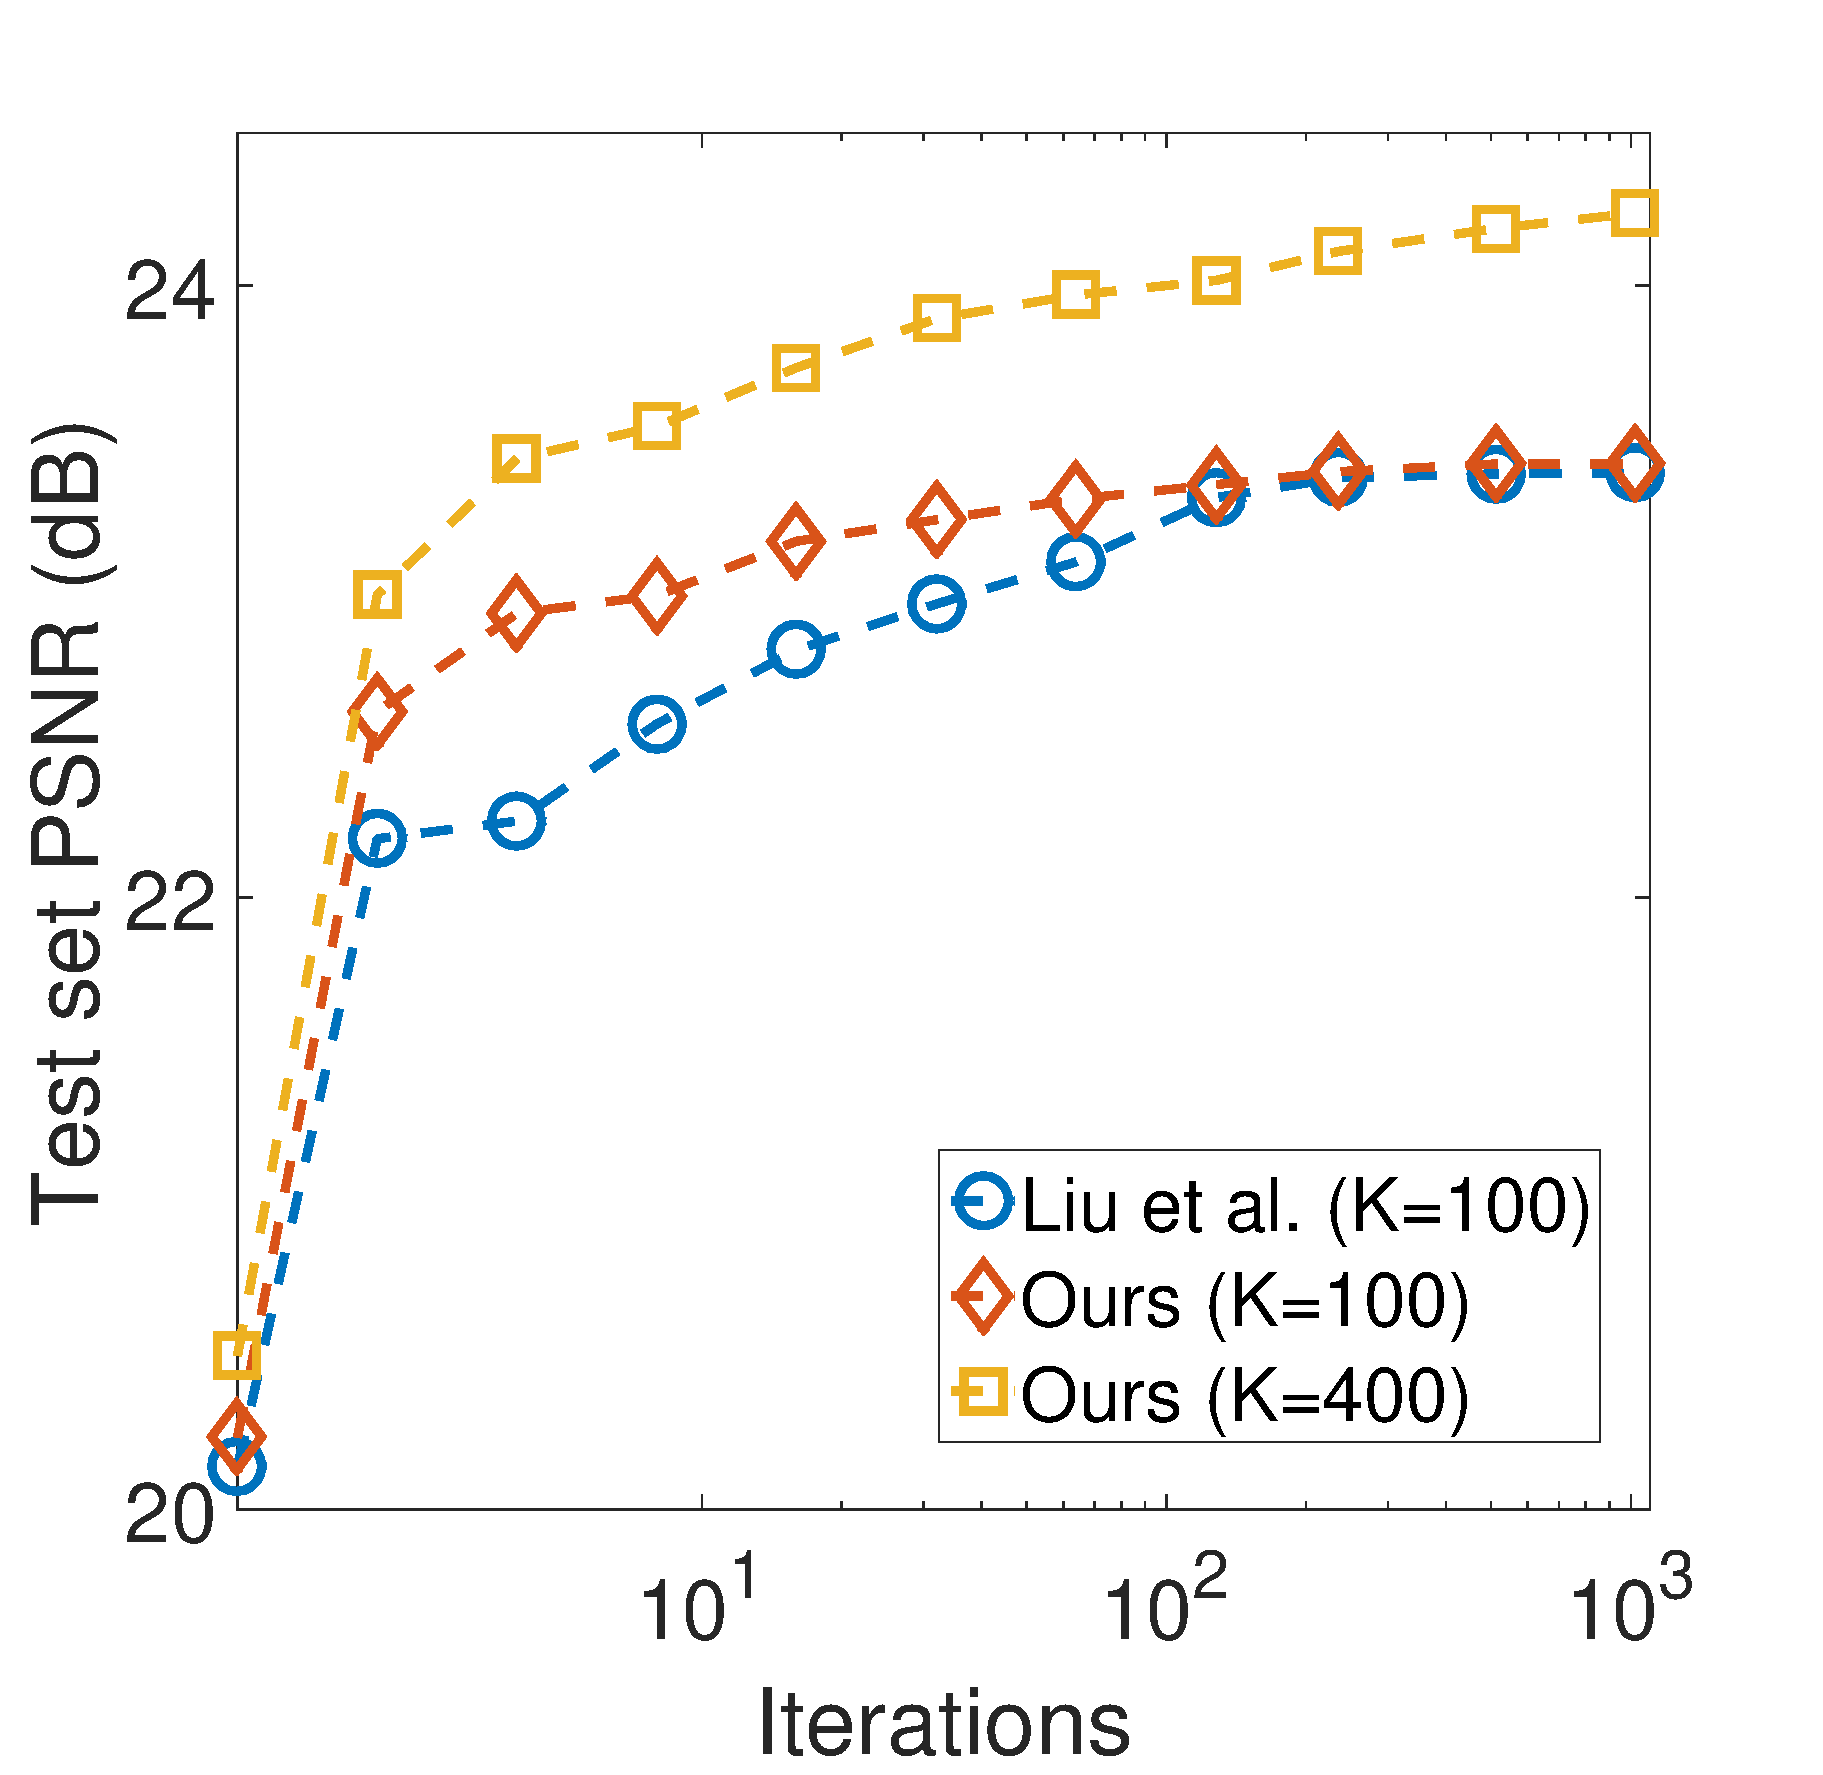
\includegraphics[width=1\linewidth]{figure/overComplete-ite.pdf}
\end{subfigure}
\begin{subfigure}{0.5\textwidth}
  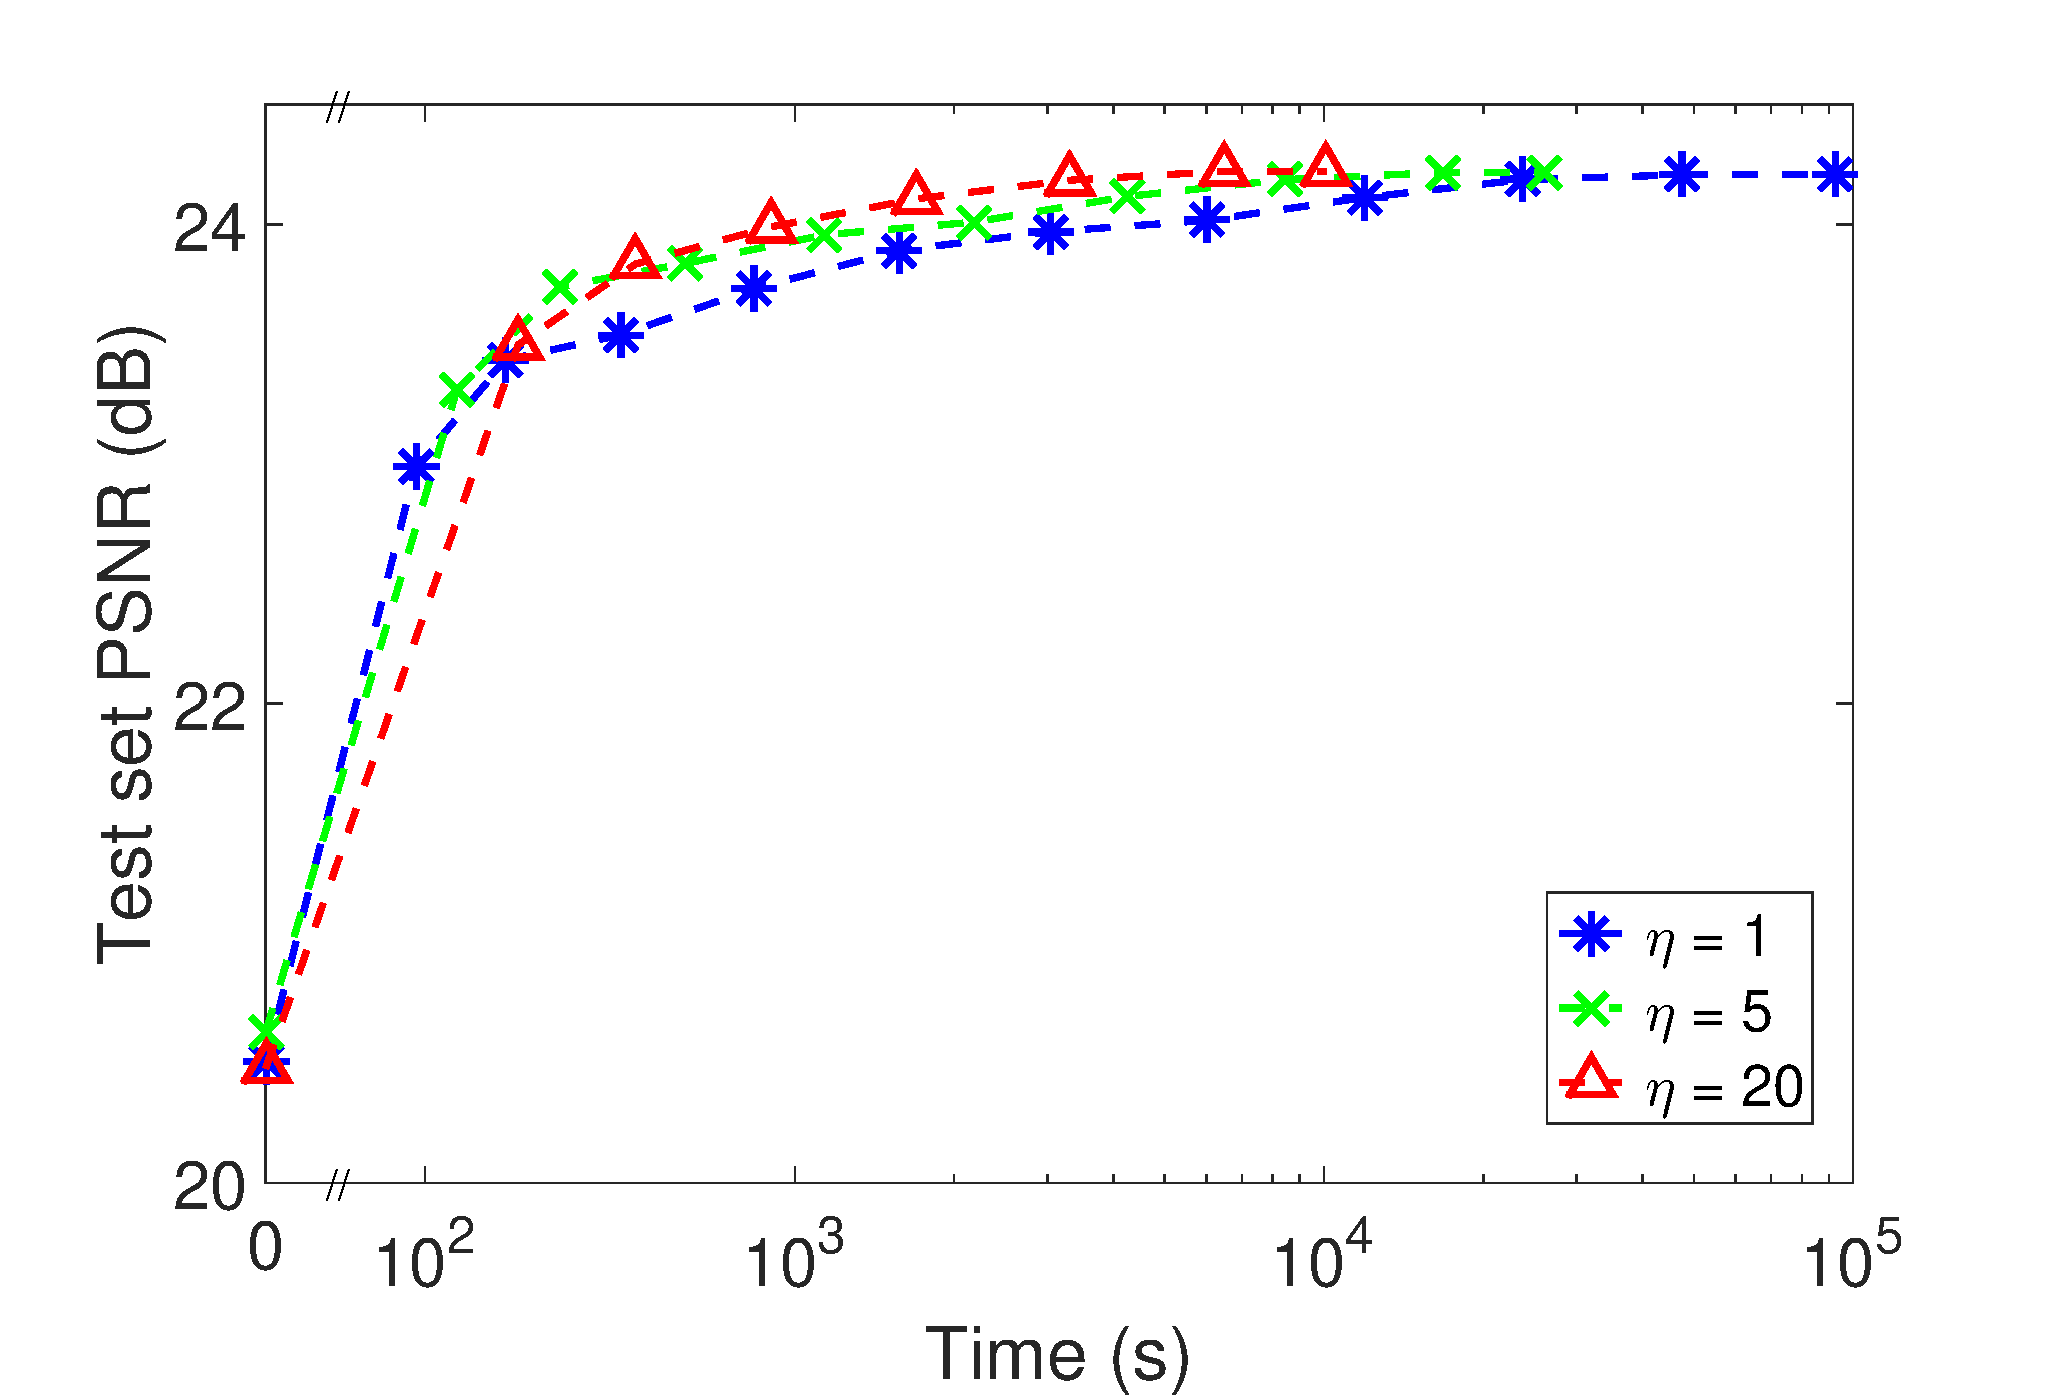
\includegraphics[width=1\linewidth]{figure/minibatch.pdf}
\end{subfigure}

\caption{Top: Testing PSNR for the comparable method~\cite{liu-2018-first} with $K=100$, and our method (SOCSC) with $K=100$ and $K=400$, respectively. Every iteration draws a single image from those 1000 image patches. Bottom: Testing PSNR for SOCSC ($K=400$) with varying values of $\eta$. The learned filters are examined on the test sets every $2^i$ iterations and also at the last iteration, where $i=0,1,\dots$. Note that all the results are generated by a single-core program.}
\label{fig:overComDicAndMinibatch}
\end{figure}


% --- DO NOT DELETE ---
% Local Variables:
% mode: latex
% mode: flyspell
% mode: TeX-PDF
% End:



% \input{Discussions}

{\small
\bibliographystyle{ieeetr}
\bibliography{egbib}
}

\end{document}